\chapter{NCC}
Please tell more about conclusion and how to the next work of this study.

\section{Lusia Violita Aprilian-1184080}
\subsection{Teori}
\begin{enumerate}
\item Menjelaskan kenapa file teks harus dilakukan tokenizer
	\par Tokenizer adalah untuk membuat vektor dari teks. Dan mengapa harus dilakukan tokenizer? itu karena dengan memfungsikan tokenizer, teks dapat divektorkan. Sehingga teks yang telah telah divektorkan tersebut dapat terbaca pada Machine Learning.
	\par Berikut adalah ilustrasi pemakaian pada tokenizer, perhatikan gambar \ref{7A1}
		\begin{figure}[!hbtp]
		\centering
		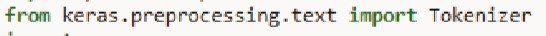
\includegraphics[scale=0.4]{figures/v1.jpg}
		\caption{Lusia-Tokenizer}
		\label{7A1}
		\end{figure}

\item Menjelaskan konsep dasar K-Fold Cross Validation
	\lstinputlisting[firstline=8, lastline=20]{src/1164080/7A2.py}
	\par Berdasarkan kode listing tersebut dapat dijelaskan bahwa :
	\begin{enumerate}
	\item Membuat variabel kfold yang memanggil fungsi StratifiedKFold. StratifiedKFold itu sendiri ialah variasi Kfold yang mengembalikan lipatan bertingkat. Yang dimana pada kode program tersebut jumlah lipatannya adalah 5 atau dibagi menjadi 5 bagian.
	\item Membuat variabel split yang mempresentasikan variabel kfold untuk dibagi berdasarkan class.
	\end{enumerate}
	
	\par Berikut adalah gambar ilustrasi dari kosep dasar kfold, perhatikan gambar \ref{7A2}.
		\begin{figure}[!hbtp]
		\centering
		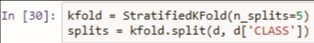
\includegraphics[scale=0.4]{figures/v2.jpg}
		\caption{Lusia-StratifiedKFold}
		\label{7A2}
		\end{figure}

\item Menjelaskan kode program for train, test in splits.
	\lstinputlisting[firstline=8, lastline=20]{src/1164080/7A3.py}
	
	\par Berdasarkan kode program tersebut, maka dapat dijelaskan bahwa kode tersebut digunakan untuk mencetak posisi pengujian pada train dan test yang telah dipisahkan. Dan memastikan bahwa kedua data tersebut tidak terjadi overlaping atau tumpang tindih dalam  setiap pemisahan.
	
	\par Berikut adalah gambar ilustrasi dari for train, test in splits, perhatikan gambar \ref{7A3a}.
	
		\begin{figure}[!hbtp]
		\centering
		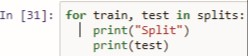
\includegraphics[scale=0.4]{figures/v3a.jpg}
		\caption{Lusia-for train, test in splits}
		\label{7A3a}
		\end{figure}
		
	\par Apabila kode program pada gambar \ref{7A3a} dijalankan, maka akan menghasilkan row\_id sebanyak 5 bagian. Dan jika diperthatikan, setiap bagian tidak terjadi pengulangan sehingga bisa bisa dibilang tidak terjadi overlaping pada data. Perhatikan gambar \ref{7A3b}.
		\begin{figure}[!hbtp]
		\centering
		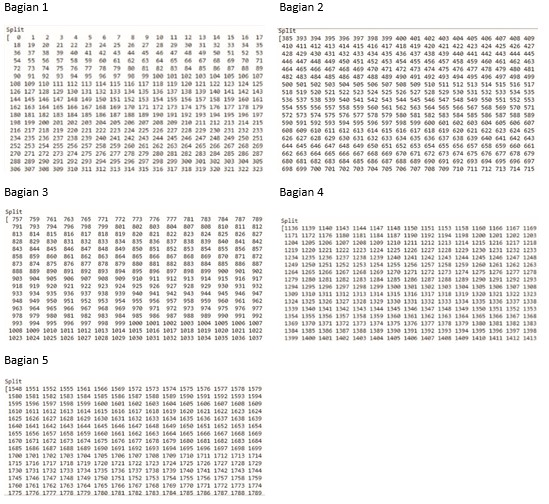
\includegraphics[scale=0.3]{figures/v3b.jpg}
		\caption{Lusia-Hasil Bagian 1}
		\label{7A3b}
		\end{figure}

\item Menjelaskan maksud kode program
	\lstinputlisting[firstline=8, lastline=20]{src/1164080/7A4.py}
	\par Dari kode program tersebut dapat dijelaskan bahwa membuat fungsi train dan test dengan menggunakan dataset yang hanya diambil kolom 'CONTENT' saja. iloc berfingsi sebagai pengindeksan posisi menggunakan integer.
	
	\par Berikut ilustrasi dari kode program tersebut, perhatikan gambar \ref{7A4}.
		\begin{figure}[!hbtp]
		\centering
		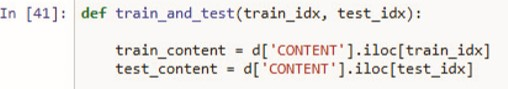
\includegraphics[scale=0.4]{figures/v4.jpg}
		\caption{Lusia-Ilustrasi Kode Program No.4}
		\label{7A4}
		\end{figure}

\item Menjelaskan maksud fungsi
	\lstinputlisting[firstline=8, lastline=20]{src/1164080/7A5.py}
		
	\par Dari kode program tersebut dapat dijelaskan bahwa pada baris pertama adalah membuat variabel tokenizer untuk memanggil fungsi tokenizer agar dapat dilakukan vektorisasi dari kata. Dimana pada kode program pada baris pertama menggunakan 2000 kata atau 2000 kolom.
	\par Sedangkan pada baris kedua dari kode program tersebut menjelaskan bahwa tokenizer difungsikan pada data train yang telah di fitting.
	
	\par Berikut adalh gambar ilustrasi dari fungsi pada kode program tersebut, perhatikan gambar \ref{7A5}.
	
		\begin{figure}[!hbtp]
		\centering
		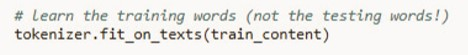
\includegraphics[scale=0.4]{figures/v5.jpg}
		\caption{Lusia-Ilustrasi Maksud fungsi No.5}
		\label{7A5}
		\end{figure}

\item Menjelaskan maksud fungsi
	\lstinputlisting[firstline=8, lastline=20]{src/1164080/7A6.py}
		
	\par Dari fungsi pada kode program tersebut dapat dijelaskan bahwa :
	\begin{enumerate}
	\item Baris pertama membuat variabel d\_train\_inputs untuk memanggil fungsi tokrnizer dan merubah data train yang berupa teks ke dalam bentuk matrix dengan menggunakan model tfidf.
	\item Baris kedua membuat variabel d\_test\_inputs untuk memanggil fungsi tokrnizer dan merubah data test yang berupa teks ke dalam bentuk matrix dengan menggunakan model tfidf.
	\end{enumerate}
	
	\par Berikut adalah gambar ilustrasi dari fungsi pada kode program tersebut, perhatikan gambar \ref{7A6}.
	
		\begin{figure}[!hbtp]
		\centering
		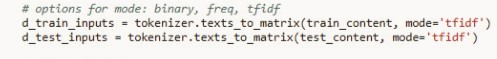
\includegraphics[scale=0.4]{figures/v6.jpg}
		\caption{Lusia-Ilustrasi Maksud fungsi No.6}
		\label{7A6}
		\end{figure}
		
\item Menjelaskan maksud fungsi
	\lstinputlisting[firstline=8, lastline=20]{src/1164080/7A7.py}
		
	\par Dari fungsi pada kode program tersebut dapat dijelaskan bahwa fungsi tersebut akan membagi matrix tfidf tadi dengan amax yaitu mengembalikan maksimum array atau maksimum sepanjang sumbu. Yang hasilnya akan dimasukan kedalam variabel d\_train\_inputs untuk data train dan d\_test\_inputs untuk data test dengan nominal absolut atau tanpa ada bilangan negatif dan koma.
	
	\par Berikut adalah gambar ilustrasi dari fungsi pada kode program tersebut, perhatikan gambar \ref{7A7}.
	
		\begin{figure}[!hbtp]
		\centering
		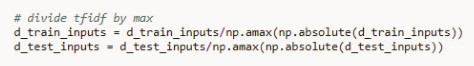
\includegraphics[scale=0.4]{figures/v7.jpg}
		\caption{Lusia-Ilustrasi Maksud fungsi No.7}
		\label{7A7}
		\end{figure}
	
\item Menjelaskan maksud fungsi
	\lstinputlisting[firstline=8, lastline=20]{src/1164080/7A8.py}
		
	\par Dari fungsi pada kode program tersebut dapat dijelaskan bahwa fungsi tersebut ditujukan untuk melakukan one-hot encoding supaya bisa masuk dan digunakan pada neural network. One-hot encoding diambil dari 'CLASS' yang berarti hanya terdapat 2 neuron, yaitu satu nol(1,0) atau nol satu(0,1) karena pilihannya hanya ada dua (spam atau bukan).
	\par Berikut adalah gambar ilustrasi dari fungsi pada kode program tersebut, perhatikan gambar \ref{7A8}.
		\begin{figure}[!hbtp]
		\centering
		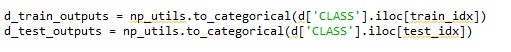
\includegraphics[scale=0.4]{figures/v8.jpg}
		\caption{Lusia-Ilustrasi Maksud fungsi No.8}
		\label{7A8}
		\end{figure}

\item Menjelaskan maksud fungsi
	\lstinputlisting[firstline=8, lastline=20]{src/1164080/7A9.py}
	\par Dari fungsi pada kode program tersebut ditujukan untuk melakukan pemodelan dengan sequential, membandingkan setiap satu larik elemen dengan cara satu persatu secara beruntun. Dimana terdapat 512 neuron inputan dengan input shape 2000 vektor yang sudah dinormalisasi. Lalu model dilakukan aktivasi dengan fungsi 'relu'. Kemudian dilakukan pemotongan bobot supaya tidak overfitting sebesar 50 persen dari neuron inputan 512. Lalu pada layer output terdapat 2 neuron outputan yaitu nol(1,0) atau nol satu(0,1). Kemudian outputan tersebut diaktivasi menggunakan fungsi softmax (mencari nilai maximal).
	\par Berikut adalah gambar ilustrasi dari fungsi pada kode program tersebut, perhatikan gambar \ref{7A9}.
		\begin{figure}[!hbtp]
		\centering
		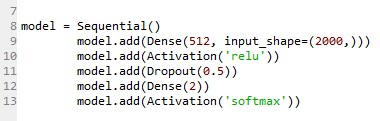
\includegraphics[scale=0.4]{figures/v9.jpg}
		\caption{Lusia-Ilustrasi Maksud fungsi No.9}
		\label{7A9}
		\end{figure}
		
\item Menjelaskan maksud fungsi
	\lstinputlisting[firstline=8, lastline=20]{src/1164080/7A10.py}
	\par Dari fungsi pada kode program tersebut model yang telah dibuat selanjutnya dicompile dengan menggunakan algoritma optimisasi, fungsi loss, dan fungsi metrik.
	\par Berikut adalah gambar ilustrasi dari fungsi pada kode program tersebut, perhatikan gambar \ref{7A10}.
		\begin{figure}[!hbtp]
		\centering
		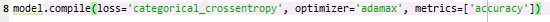
\includegraphics[scale=0.4]{figures/v10.jpg}
		\caption{Lusia-Ilustrasi Maksud fungsi No.10}
		\label{7A10}
		\end{figure}

\item Menjelaskan apa itu Deep Learning
	\par Deep Learning merupakan cabang dari Machine Learning atau bagian keluarga yang lebih luas dari method machine learning berdasarkan pada representasi data pembelajaran. Deep Learning menggunakan Deep Neural Network dalam menyelesaikan suatu masalah yang terjadi pada Machine Learning.
	
\item Menjelaskan apa itu Deep Neural dan bedanya dengan Deep Learning
	\par Deep Neural Network atau DNN merupakan algoritma yang berbasis neural network yang digunakan untuk mengambil keputusan.
	\par Yang membedakan Deep Learning dengan  Deep Neural Network (DNN) adalah DNN merupakan algoritma yang digunakan pada Deep Learning, sedangkan Deep Learning merupakan model yang menggunakan algoritma DNN.
	
\item Menjelaskan perhitungan algoritma konvolusi
	\par Konvolusi pada sebuah gambar dilakukan dalam image processing untuk menerapkan operator yang mempunyai nilai output dari piksel gambar yang berasal dari kombinasi linear nilai input piksel tertentu pada gambar. 
	\par Karena NPM saya 1164080 dan hasil dari (NPM mod 3)+1 = 3, maka saya menggunaan matrik kernel berukuran 3x3. Sehingga ilustrasi gambar yang digunakan adalah seperti gambar \ref{7A13}. Misalkan  f(x,y) yang digunakan berukuran 5x5 dan kernel atau mask berukuran 3x3 masing-masing adalah sebagai berikut: 
		\begin{figure}[!hbtp]
		\centering
		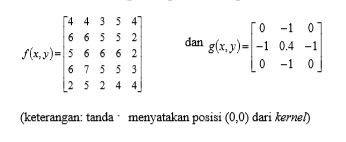
\includegraphics[scale=0.4]{figures/v13.jpg}
		\caption{Lusia-Ilustrasi Gambar}
		\label{7A13}
		\end{figure}
	\par Penyelesaian dari operasi konvolusi antara  f(x,y) dengan kernel g(x,y) pada gambar \ref{7A13} adalah  f(x,y) * g(x,y) dengan ilustrasi sebagai berikut :
	\begin{enumerate}
	\item Tempatkan matrik kernel di sebelah kiri atas, lalu hitung nilai piksel pada posisi (0,0) dari kernel tersebut seperti gambar \ref{7A13a}.
		\begin{figure}[!hbtp]
		\centering
		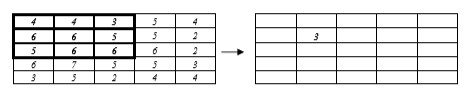
\includegraphics[scale=0.4]{figures/v13a.jpg}
		\caption{Lusia-Ilustrasi konvolusi 1}
		\label{7A13a}
		\end{figure}
		\par Konvolusi dihitung dengan cara berikut :
		\par (0x4) + (-1x4) + (0x3) + (-1x6) + (4x6) + (-1x5) + (0x5) + (-1x6) + (0x6)
		\par Sehingga didapat hasil konvolusi = 3
	\item Lalu geser kernel satu piksel ke kanan kemudian hitung kembali  nilai piksel pada posisi (0,0) dari kernel.
	\par Konvolusi dihitung dengan cara berikut :
	\par (0x4) + (-1x3) + (0x5) + (-1x6) + (4x5) + (-1x5) + (0x6) + (-1x6) + (0x6)  
	\par Sehingga didapat hasil konvolusi = 0 seperti pada gambar \ref{7A13b}.
		\begin{figure}[!hbtp]
		\centering
		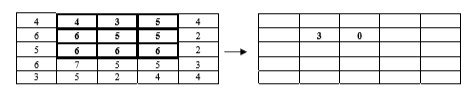
\includegraphics[scale=0.4]{figures/v13b.jpg}
		\caption{Lusia-Ilustrasi konvolusi 2}
		\label{7A13b}
		\end{figure}
		
	\item Lalu geser kernel satu piksel ke kanan kemudian hitung kembali  nilai piksel pada posisi (0,0) dari kernel.
	\par Konvolusi dihitung dengan cara berikut :
	\par (0x3) + (-1x5) + (0x4) + (-1x5) + (4x5) + (-1x2) + (0x6) + (-1x6) + (0x2)  
	\par Sehingga didapat hasil konvolusi = 2 seperti pada gambar \ref{7A13c}.
		\begin{figure}[!hbtp]
		\centering
		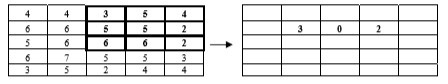
\includegraphics[scale=0.4]{figures/v13c.jpg}
		\caption{Lusia-Ilustrasi konvolusi 3}
		\label{7A13c}
		\end{figure}
		
	\item Kemudian geser matriks kernel kebawah, lalu mulai hitung kembali dari sisi kiri. Setiap kali perhitungan konvolusi dilakukan, geser matriks kernel atau piksel ke kanan seperti pada gambar \ref{7A13d}, \ref{7A13e}, dan \ref{7A13f}.
	\begin{itemize}
	\item Konvolusi pada gambar \ref{7A13d} dihitung dengan cara berikut :
	\par (0x6) + (-1x6) + (0x5) + (-1x5) + (4x6) + (-1x6) + (0x6) + (-1x7) + (0x5)   
	\par Sehingga didapat hasil konvolusi = 0 seperti pada gambar \ref{7A13d}.
		\begin{figure}[!hbtp]
		\centering
		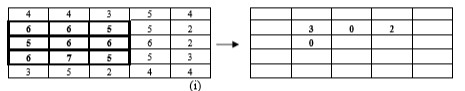
\includegraphics[scale=0.4]{figures/v13d.jpg}
		\caption{Lusia-Ilustrasi konvolusi 4}
		\label{7A13d}
		\end{figure}
	\item Konvolusi pada gambar \ref{7A13e} dihitung dengan cara berikut :
	\par (0x6) + (-1x5) + (0x5) + (-1x6) + (4x6) + (-1x6) + (0x7) + (-1x5) + (0x5)   
	\par Sehingga didapat hasil konvolusi = 2 seperti pada gambar \ref{7A13e}.
		\begin{figure}[!hbtp]
		\centering
		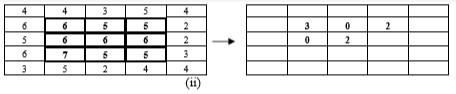
\includegraphics[scale=0.4]{figures/v13e.jpg}
		\caption{Lusia-Ilustrasi konvolusi 5}
		\label{7A13e}
		\end{figure}
		
	\item Konvolusi pada gambar \ref{7A13f} dihitung dengan cara berikut :
	\par (0x5) + (-1x5) + (0x2) + (-1x6) + (4x6) + (-1x2) + (0x5) + (-1x5) + (0x3)    
	\par Sehingga didapat hasil konvolusi = 6 seperti pada gambar \ref{7A13f}.
		\begin{figure}[!hbtp]
		\centering
		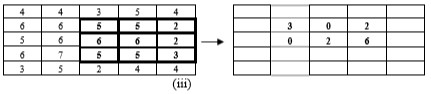
\includegraphics[scale=0.4]{figures/v13f.jpg}
		\caption{Lusia-Ilustrasi konvolusi 6}
		\label{7A13f}
		\end{figure}
	\end{itemize}		
	\item Dengan langkah-langkah yang sama, piksel-piksel pada baris ketiga dilakukan orerasi konvolusi sehingga menghasilkan seperti gambar \ref{7A13g}.
		\begin{figure}[!hbtp]
		\centering
		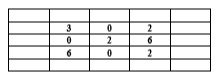
\includegraphics[scale=0.4]{figures/v13g.jpg}
		\caption{Lusia-Ilustrasi konvolusi baris ketiga}
		\label{7A13g}
		\end{figure}
	\par Apabila nilai piksel hasil konvolusi adalah negatif, maka nilai tersebut dijadikan 0. Sebaliknya, bila nilai piksel hasil konvolusi lebih besar dari nilai kabuan maksimum (255), maka nilai tersebut dijadikan ke nilai keabuan maksimum.
	
	\end{enumerate}

\end{enumerate}

\subsection{Cek Plagiarisme}
\par Dari hasil kerja pada chapter 7, jika dicek plagiarisme menghasilkan seperti gambar \ref{7D1}.
		\begin{figure}[!hbtp]
		\centering
		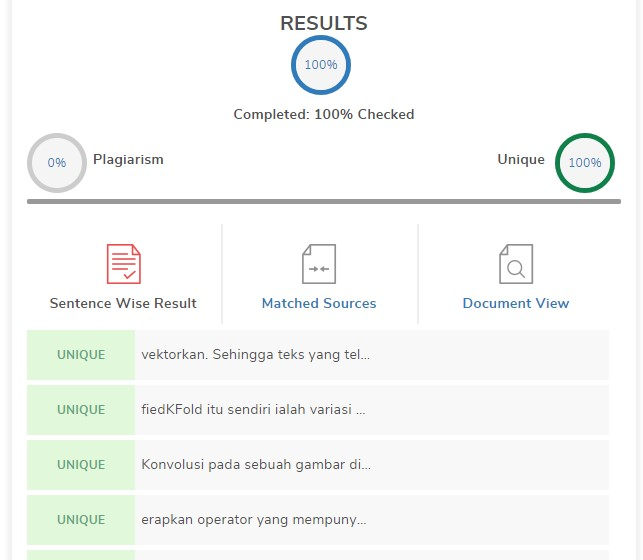
\includegraphics[scale=0.4]{figures/pc7.jpg}
		\caption{Lusia-Plagiarisme}
		\label{7D1}
		\end{figure}




\section{Rahmi Roza-1164085}
\subsection{Teori}
\begin{enumerate}
\item Kenapa File Suara Harus Dilakukan Tokenizer
\begin{itemize}
\item Penjelasan: Untuk membedakan karakter-karakter tertentu dalam suatu teks dan juga sebagai pemisah kata atau bukan.Tokenizer dilakukan dengan cara melakukan pemotongan string input berdasarkan tiap kata yang menyusunnya.
\par 
\par
\item Ilustrasi Gambar
\item Tokenizer \ref{teori1}
\begin{figure}[!hbtp]
\centering
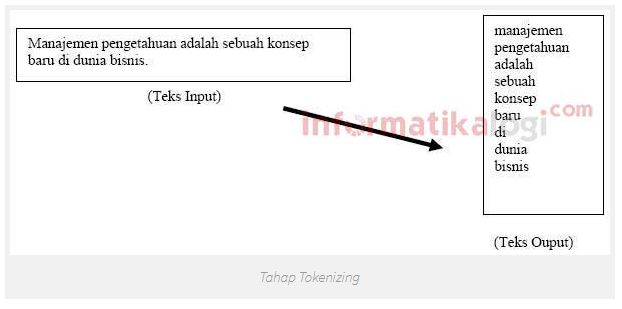
\includegraphics[scale=0.7]{figures/teori1.jpg}
\caption{Tokenizer Roza}
\label{teori1}
\end{figure}
\par
\end{itemize}
\par
\par

\item Jelaskan konsep dasar K Fold Cross Validation pada dataset komentar Youtube pada kode listing 
\lstinputlisting[firstline=8, lastline=20]{src/1164085/chapter7-2.py}
\begin{itemize}
\item Penjelasan: Startified KFold berisikan presentasi sampel untuk setiap kelas. Dimana dalam ilustrasi ini sampel dibagi menjadi 5 dalam setiap class nya. Kemudian sampel tadi akan dimasukan kedalam class dari dataset youtube tadi.
\par 
\par
\item Ilustrasi Gambar
\item K-Fold Cross Validation \ref{teori2}
\begin{figure}[!hbtp]
\centering
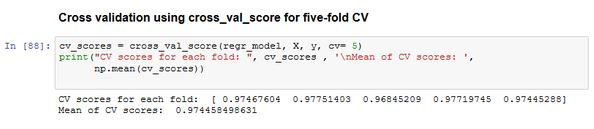
\includegraphics[scale=0.7]{figures/teori2.jpg}
\caption{K-Fold Cross Validation Roza}
\label{teori2}
\end{figure}
\par
\end{itemize}
\par
\par

\item Jelaskan apa maksudnya kode program for train, test in splits.dilengkapi dengan ilustrasi atau gambar.
\begin{itemize}
\item Penjelasan: Maksudnya yaitu untuk menguji apakah setiap data pada dataset sudah di split dan tidak terjadi penumpukan. Yang dimana maksudnya di setiap class tidak akan muncul id yang sama. Ilustrasinya misalkan kita memiliki 4 botol minuman dengan model yang berbeda. Kemudian kita bagikan kedua anak, tentunya setiap anak yang menerima botol tidak memiliki botol minuman  yang sama modelnya.
\par 
\par
\item Ilustrasi Gambar
\item No 3  \ref{teori3}
\begin{figure}[!hbtp]
\centering
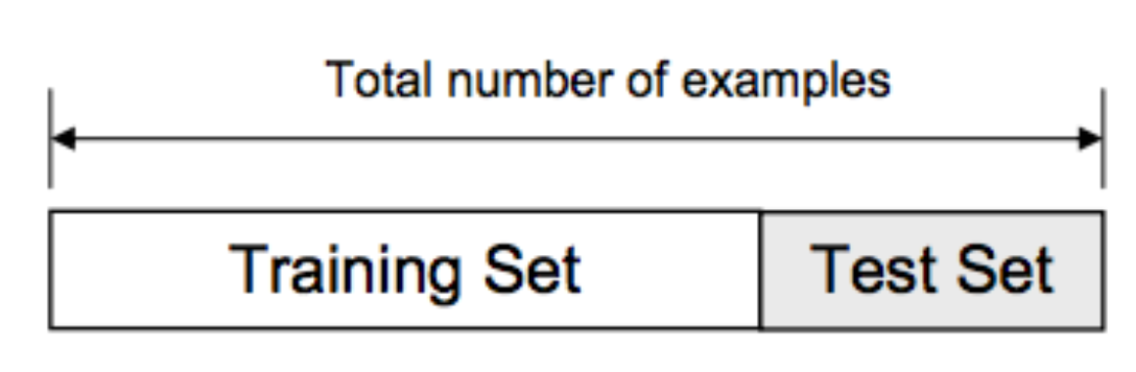
\includegraphics[scale=0.2]{figures/teori3.png}
\caption{No 3 Roza}
\label{teori3}
\end{figure}
\par
\end{itemize}
\par
\par

\item Jelaskan apa maksudnya kode program {train\_content = d['CONTENT'].iloc[train\_idx]} dan {test\_content = d['CONTENT'].iloc[test\_idx]}.
\begin{itemize}
\item Penjelasan: Maksudnya yaitu mengambil data pada kolom atau index CONTENT yang merupakan bagian dari train\_idx dan test\_idx. Ilustrasinya, ketika data telah diubah menjadi train dan test maka kita dapat memilihnya untuk ditampilkan pada kolom yang diinginkan.
\par 
\par
\end{itemize}
\par
\par

\item Jelaskan apa maksud dari fungsi tokenizer {tokenizer = Tokenizer(num\_words=2000)} dan tokenizer.{tokenizer.fit\_on\_texts(train\_content)}, dilengkapi dengan ilustrasi atau gambar.
\begin{itemize}
\item Penjelasan: Dimana variabel tokenizer akan melakukan vektorisasi kata menggunakan fungsi Tokenizer yang dimana jumlah kata yang ingin diubah kedalam bentuk token adalah 2000 kata. Dan untuk \emph{tokenizer.fit\_on\_texts(train\_content)} maksudnya kita akan melakukan fit tokenizer hanya untuk data trainnya saja tidak dengan data test nya untuk kolom CONTENT. 
\par 
\par
\item Ilustrasi Gambar
\item No 5 \ref{teori5}
\begin{figure}[!hbtp]
\centering
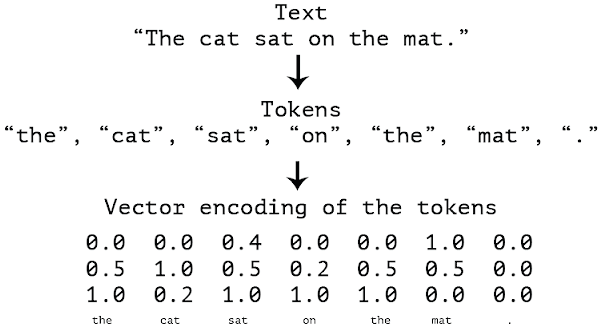
\includegraphics[scale=0.4]{figures/teori5.png}
\caption{No 5 Roza}
\label{teori5}
\end{figure}
\par
\end{itemize}
\par
\par


\item Jelaskan apa maksud dari fungsi \emph{d\_train\_inputs = tokenizer.texts\_to\_matrix(train\_content, mode='tfidf')} dan \emph{d\_test\_inputs = tokenizer.texts\_to\_matrix(test\_content, mode='tfidf')}, dilengkapi dengan ilustrasi kode dan atau gambar.
\begin{itemize}
\item Penjelasan: Maksudnya yaitu untuk variabel d\_train\_inputs akan melakukan tokenizer dari bentuk teks ke matrix dari data train\_content dengan mode matriksnya yaitu tfidf begitu juga dengan variabel d\_test\_inputs untuk data test. Berikut gambar ilustrasinya
\par 
\par
\item Ilustrasi Gambar
\item No 6 \ref{teori6}
\begin{figure}[!hbtp]
\centering
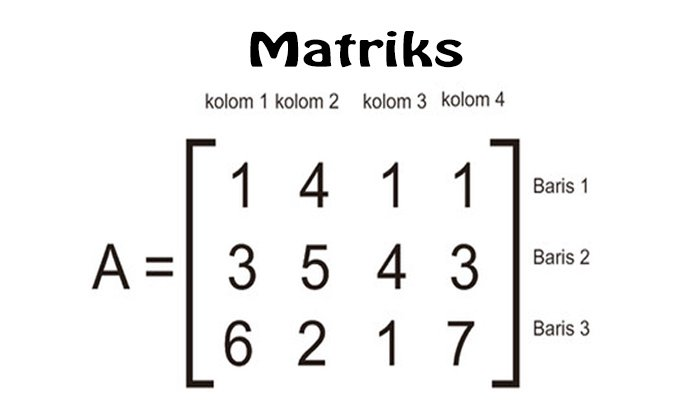
\includegraphics[scale=0.3]{figures/teori6.jpg}
\caption{No 6 Roza}
\label{teori6}
\end{figure}
\par
\end{itemize}
\par
\par

\item Jelaskan apa maksud dari fungsi \emph{d\_train\_inputs = d\_train\_inputs/np.amax(np.absolute(d\_train\_inputs))} dan \emph{d\_test\_inputs = d\_test\_inputs/np.amax(np.absolute(d\_test\_inputs))}, dilengkapi dengan ilustrasi atau gambar.
\begin{itemize}
\item Penjelasan: Fungsi tersebut akan membagi matrix tfidf tadi dengan amax yaitu mengembalikan maksimum array atau maksimum sepanjang sumbu. Yang hasilnya akan dimasukan kedalam variabel d\_train\_inputs untuk data train dan d\_test\_inputs untuk data test dengan nominal absolut atau tanpa ada bilangan negatif dan koma.
\par 
\par
\item Ilustrasi Gambar
\item No 7 \ref{teori7}
\begin{figure}[!hbtp]
\centering
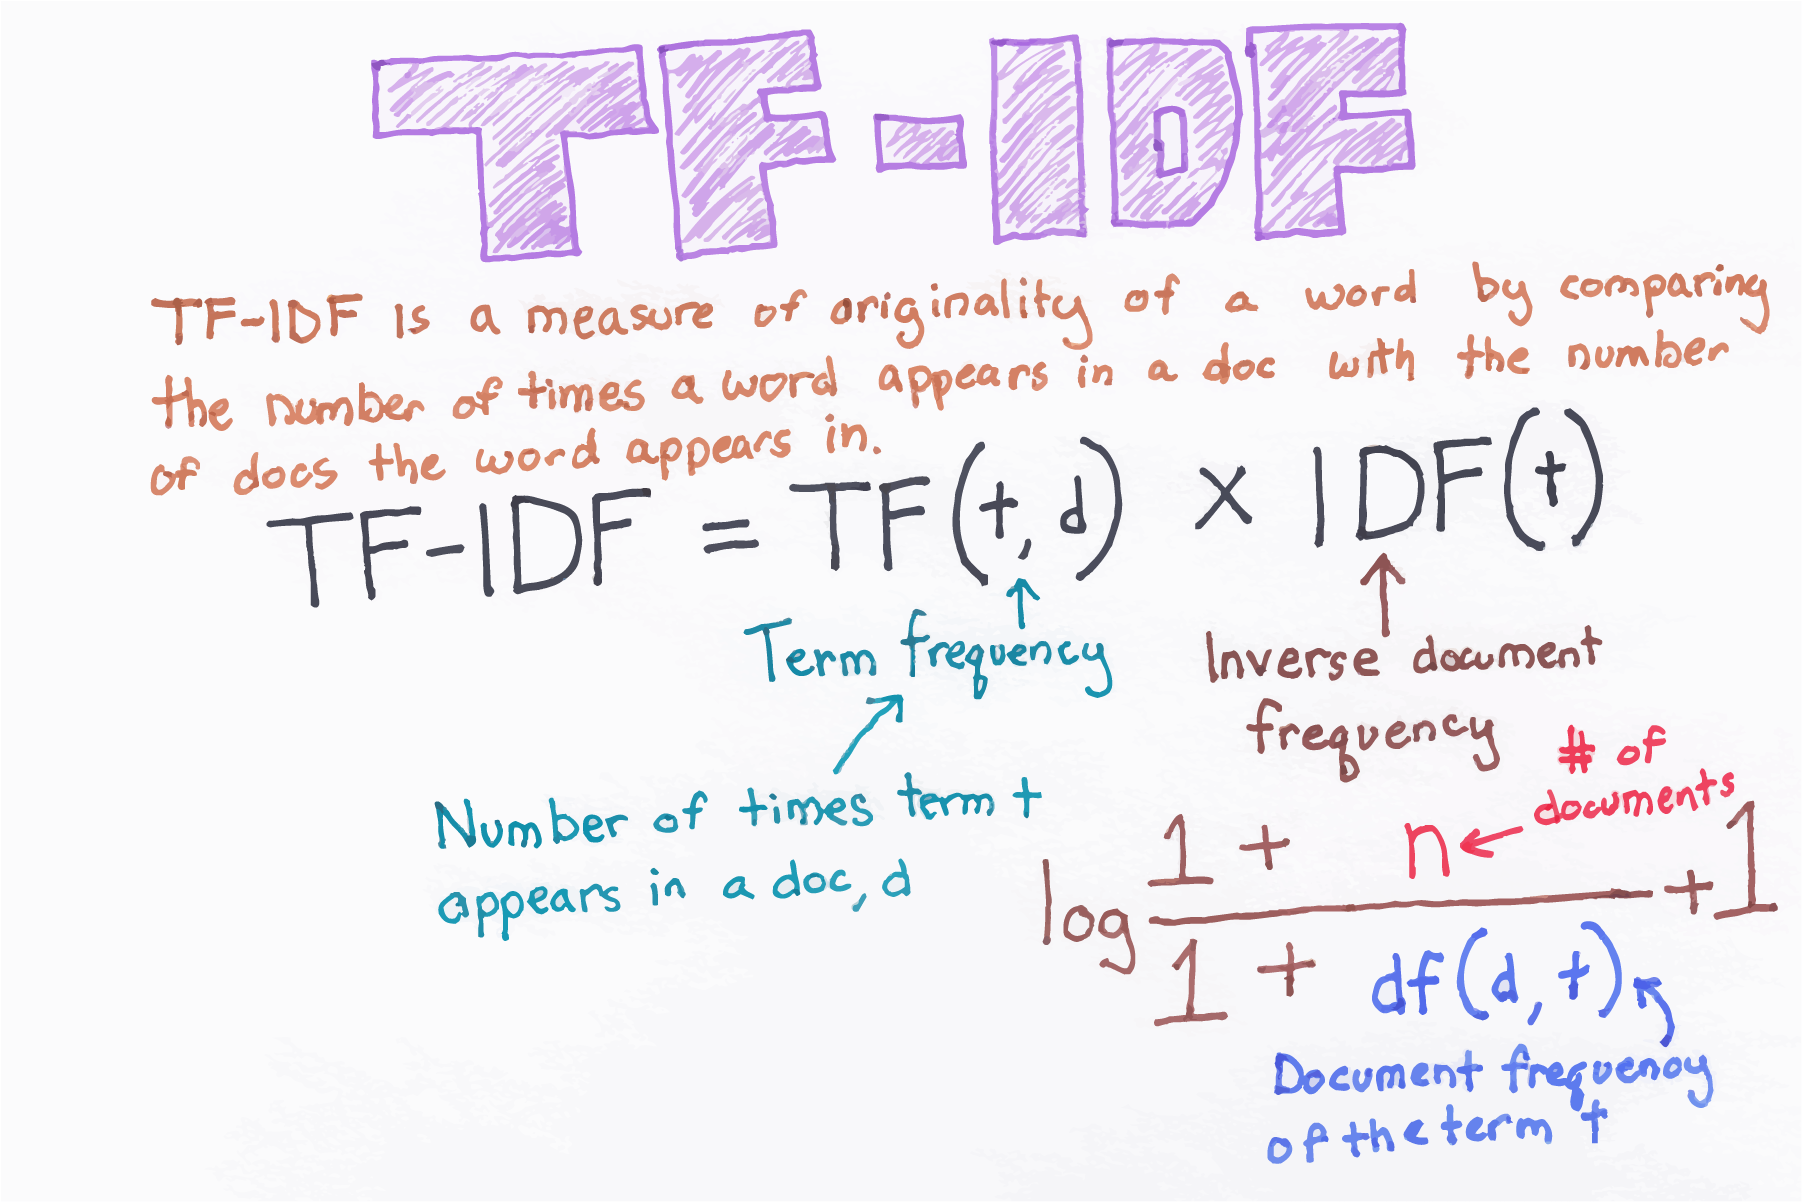
\includegraphics[scale=0.4]{figures/teori7.png}
\caption{No 7 Roza}
\label{teori7}
\end{figure}
\par
\end{itemize}
\par
\par

\item Jelaskan apa maksud fungsi dari d\_train \_outputs = np\_utils.to\_categorical(d['CLASS'].iloc[train dan d\_test \_outputs = np\_ utils.to\_categorical(d['CLASS'].iloc[test\_idx]) dalam kode program
\begin{itemize}
\item Penjelasan: Dari fungsi pada kode program tersebut dijelaskan fungsi tersebut ditujukan untuk melakukan one-hot encoding agar dapat masuk dan digunakan di neural network. One-hot encoding diambil dari 'CLASS' yang berarti hanya terdapat 2 neuron, yaitu satu nol(1,0) atau nol satu(0,1) karena pilihannya hanya ada dua (spam atau bukan).
\par 
\par
\item Ilustrasi Gambar
\item No 8 \ref{teori8}
\begin{figure}[!hbtp]
\centering
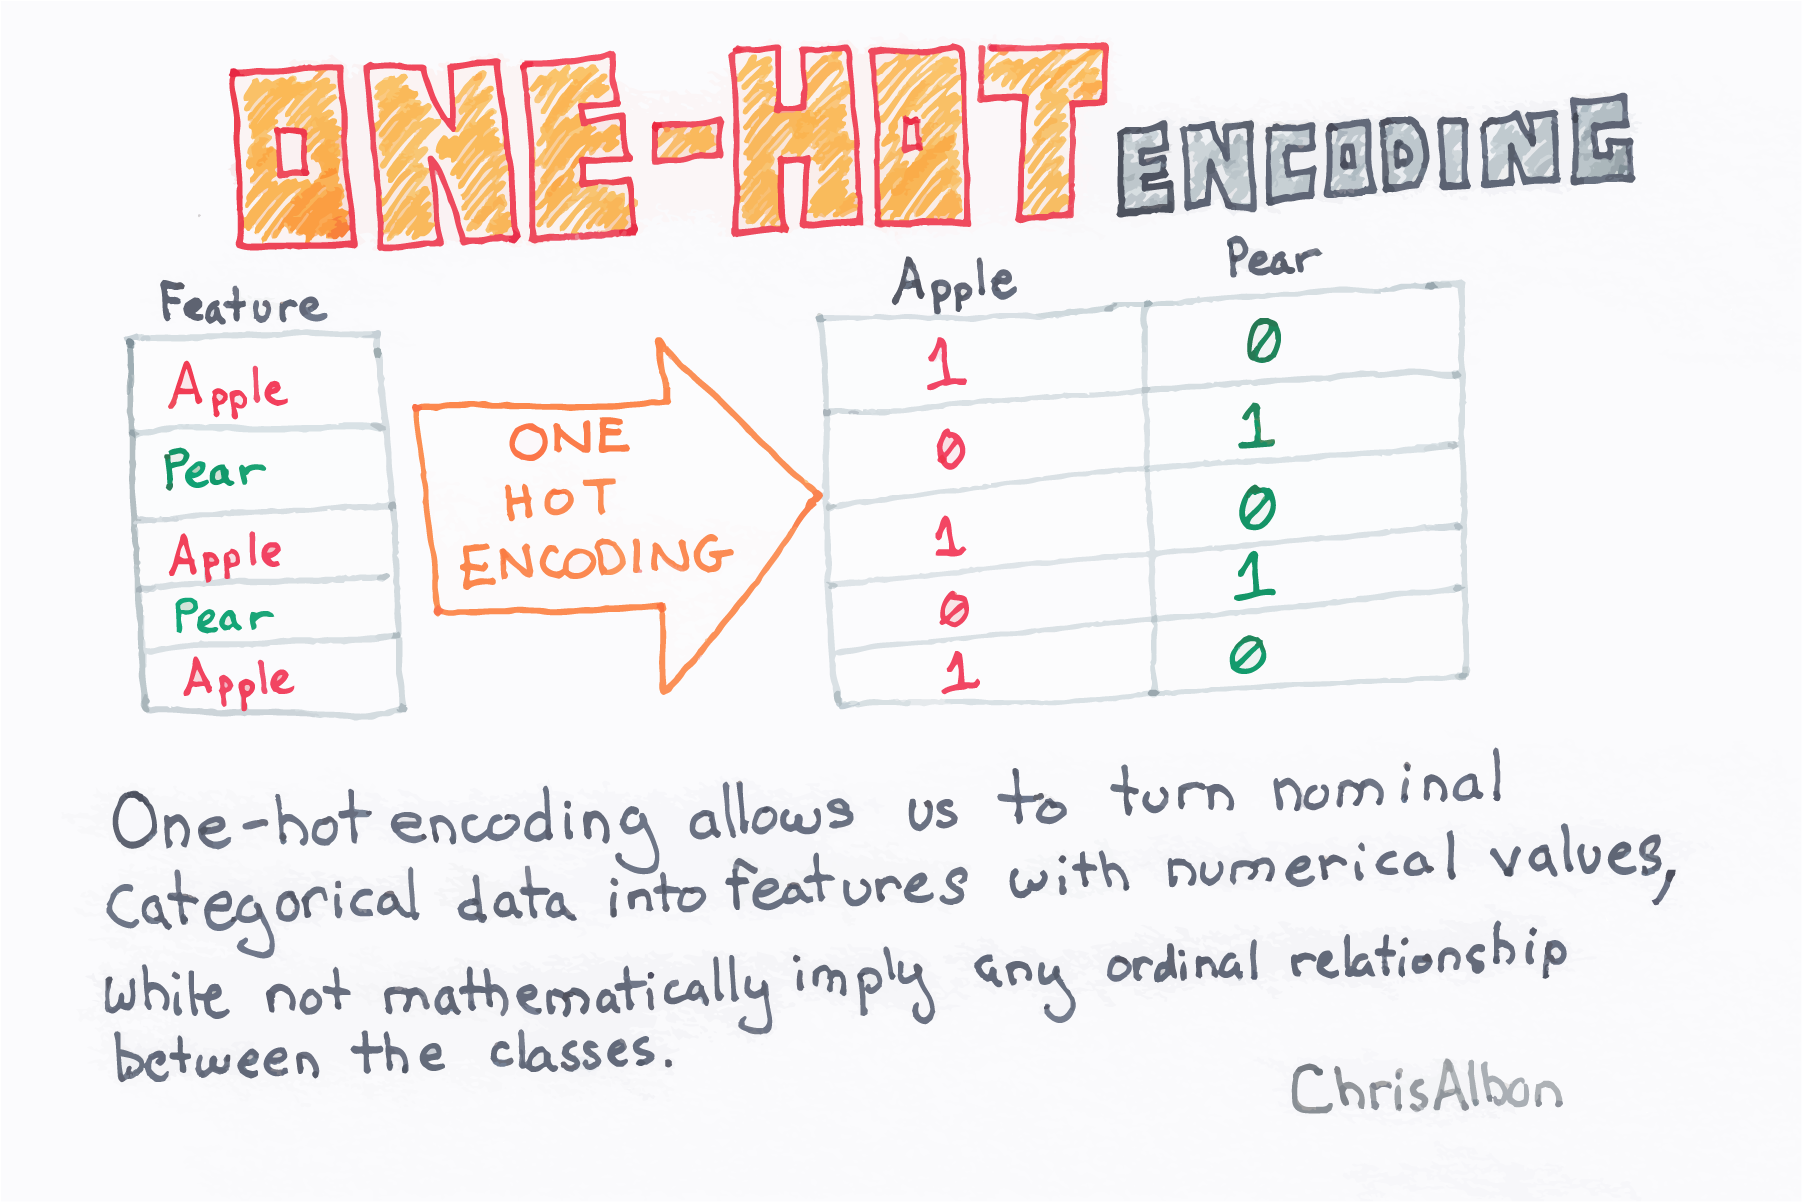
\includegraphics[scale=0.4]{figures/teori8.png}
\caption{No 8 Roza}
\label{teori8}
\end{figure}
\par
\end{itemize}
\par
\par

\item Jelaskan apa maksud dari fungsi di listing!
\lstinputlisting[firstline=8, lastline=20]{src/1164085/chapter7-9.py}
\begin{itemize}
\item Penjelasan: Dari fungsi pada kode program tersebut ditujukan untuk melakukan pemodelan dengan sequential, membandingkan setiap satu larik elemen dengan cara satu persatu secara beruntun. Dimana terdapat 512 neuron inputan dengan input shape 2000 vektor. Lalu model dilakukan aktivasi dengan fungsi 'relu'. Kemudian dilakukan pemotongan bobot supaya tidak overfitting sebesar 50 persen dari neuron inputan 512. Lalu pada layer output terdapat 2 neuron outputan yaitu nol(1,0) atau nol satu(0,1). Kemudian outputan tersebut diaktivasi menggunakan fungsi softmax.
\par 
\end{itemize}
\par
\par

\item Jelaskan apa maksud dari fungsi di listing!
\lstinputlisting[firstline=8, lastline=20]{src/1164085/chapter7-10.py}
\begin{itemize}
\item Penjelasan: Dari fungsi pada kode program tersebut model yang telah dibuat selanjutnya dicompile dengan menggunakan algoritma optimisasi denganfungsi fungsi loss, fungsi opttimaizer dan fungsi metrik. Dimana nama masing-masing fungsi tersebut adalah categorical\_crossentropy, adamax dan accuracy.
\par 
\end{itemize}
\par
\par

\item 	Apa Itu Deep Learning
\begin{itemize}
\item Penjelasan: 
\par  Deep learning merupakan sub bidang pembelajaran mesin yang berkaitan dengan algoritma.
\end{itemize}
\par
\par

\item Apa itu Deep Neural Network Dan Apa Bedanya Dengan Deep Learning :
\begin{itemize}
\item Penjelasan Deep Neural Network : 
\par  Deep neural network adalah jaringan syaraf dengan tingkat kompleksitas tertentu, jaringan syaraf dengan lebih dari dua lapisan.
\par
\item Perbedaan Deep Neural Network Dan Deep Learning :
\par Perbedaan antara deep neural network dan deep learning terletak pada kedalaman model. deep learning adalah frasa yang digunakan untuk jaringan saraf yang kompleks. Kompleksitas ini disebabkan oleh pola yang rumit tentang bagaimana informasi dapat mengalir di seluruh model.
\end{itemize}
\par
\par

\item Perhitungan Algoritma Konvolusi Dengan NPM 1164085. Seperti gambar di bawah penyelesaiannya:
\begin{itemize}
\item Ilustrasi Gambar
\item No 13 \ref{teori13}
\begin{figure}[!hbtp]
\centering
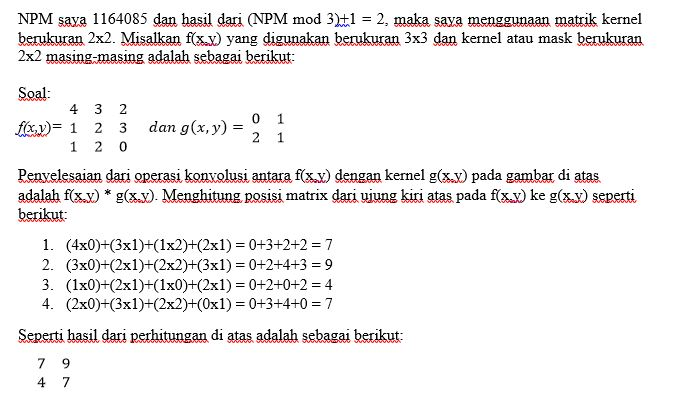
\includegraphics[scale=0.6]{figures/teori13.jpg}
\caption{No 13 Roza}
\label{teori13}
\end{figure}
\par
\end{itemize}
\par
\par
\item Plagiarisme Roza
\begin{figure}[!hbtp]
\centering
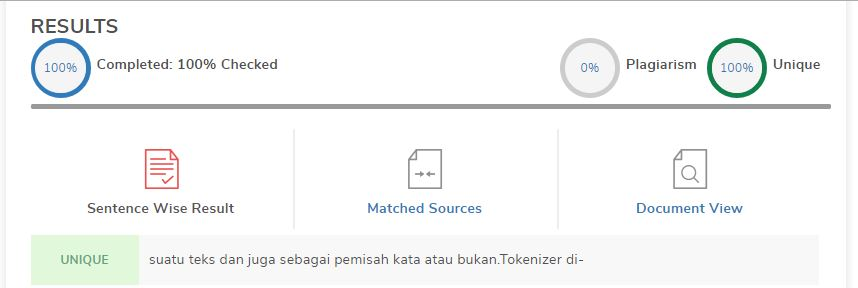
\includegraphics[scale=0.6]{figures/plagairismerozac7.jpg}
\caption{Plagiarisme Roza}
\label{teori13}
\end{figure}
\par
\end{enumerate}
\par
\par

\subsection{Praktek}
\begin{enumerate}
\item Jelaskan kode program pada blok \# In[1].
\begin{itemize}
\item Kode Program:
\lstinputlisting[firstline=1, lastline=19, caption=Praktek1.py, label={lst:import}]{src/1164085/prak1-roza.py}
\par Hasil \ref{in1roza} :
\begin{figure}[!hbtp]
\centering
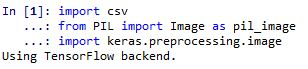
\includegraphics[scale=0.7]{figures/prak1roza.jpg}
\caption{In 1 Roza}
\label{in1roza}
\end{figure}
\par Baris 1: Mengimpoer file csv.
\par Baris 2: Dari library PIL impor gambar sebagai pil\_image.
\par Baris 3: Impor fungsi fungsi keras.processing.image
\end{itemize}
\par

\item Jelaskan kode program pada blok \# In[2].
\begin{itemize}
\item Kode Program:
\lstinputlisting[firstline=1, lastline=19, caption=Praktek2.py, label={lst:import}]{src/1164085/prak2-roza.py}
\par Hasil \ref{in2roza} :
\begin{figure}[!hbtp]
\centering
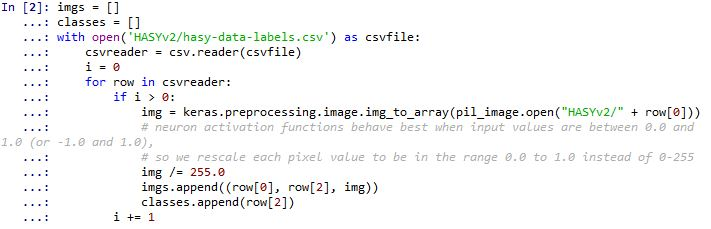
\includegraphics[scale=0.7]{figures/prak2roza.jpg}
\caption{In 2 Roza}
\label{in2roza}
\end{figure}
\par Baris 1: Membuat variabel images tanpa parameter, karena di dalam kurung kosong tanpa ada parameter yang diisi.
\par Baris 2: Membuat variabel class tanpa parameter juga karna tiada ada parameter di dalam kurung.
\par Baris 3: Membuka file HASYv2/hasy-data-labels.csv sebagai csvfile.
\par Baris 4: Membuat variabel csvreader yang memfungsikan pembacaan dari file csv yang dimasukkan
\par Baris 5: Membuat variabel i dengan parameter 0
\par Baris 6: Mengeksekusi data dari baris di pembacaan file csv.
\par Baris 7: Menggunakan perintah "if" dengan ketentuan variabel i lebih besar dari  0.
\par Baris 8: Membuat variabel img dengan nama keras.processing yang mengubah image menjadi bentuk array (bilangan) dari file HASYv2 yang dibuka dengan row berparameter 0.
\par Baris 9: Membuat variabel img tidak sama dengan 255.0
\par Baris 10: Mendefinisikan fungsi imgs.append dimana merupakan proses menggabungkan data dengan file lain  yang ditentukan dengan 3 parameter yaitu row[0], row[2] dan variabel img.
\par Baris 11: Mendefinisikan fungsi append kembali dari variabel classes dengan parameternya row[2].
\par Baris 12: Mendefinisikan fungsi dimana i variabel i akan ditambah nilainya sehingga akan bernilai 1 ( Contoh nilai i=0 dengan adanya penambahan maka hasilnya akan menjadi 1 )
\end{itemize}
\par


\item Jelaskan kode program pada blok \# In[3].
\begin{itemize}
\item Kode Program:
\lstinputlisting[firstline=1, lastline=19, caption=Praktek3.py, label={lst:import}]{src/1164085/prak3-roza.py}
\par Hasil \ref{in3roza} :
\begin{figure}[!hbtp]
\centering
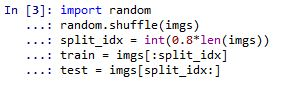
\includegraphics[scale=0.7]{figures/prak3roza.jpg}
\caption{In 3 Roza}
\label{in3roza}
\end{figure}
\par Baris 1: Import modul random
\par Baris 2: Melakukan pengocokan terhadap modul dengan parameter dimana variabelnya imgs
\par Baris 3: Membagi dan memecah index dalam bentuk integer dengan mengkalikan nilai 0.8 dengan fungsi len yang mengembalikan jumlah item dari variabel imgs.
\par Baris 4: Membuat variabel train yang mengeksekusi imgs dengan pemecahan index pada data awa.l
\par Baris 5: Membuat variabel test yang mengeksekusi imgs dengan pemecahan index pada dataakhir.

\end{itemize}
\par

\item Jelaskan kode program pada blok \# In[4].
\begin{itemize}
\item Kode Program:
\lstinputlisting[firstline=1, lastline=19, caption=Praktek4.py, label={lst:import}]{src/1164085/prak4-roza.py}
\par Hasil \ref{in4roza} :
\begin{figure}[!hbtp]
\centering
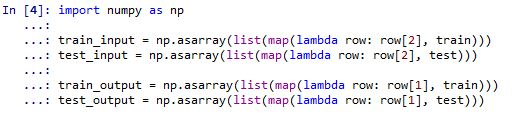
\includegraphics[scale=0.7]{figures/prak4roza.jpg}
\caption{In 4 Roza}
\label{in4roza}
\end{figure}
\par Baris 1: Import library numpy sebagai np.
\par Baris 2: Membuat variabel train\_input dimana mengubah input menjadi sebuah array dari np dengan menggunakan fungsi list untuk mengkoleksikan data yang dipilih dan dapat diubah. Didalamnya diterapkan fungsi map untuk mengembalikan iterator dari datanya dengan memfungsikan lamda pada row dengan parameter [2] untuk membuat objek fungsi menjadi lebih kecil dan mudah dieksekusi dari variabel train.
\par Baris 3:Membuat variabel test\_input dengan fungsi yang sama seperti train\_input yang membedakan hanya datanya / inputan yang diproses berasal dari variabel test
\par Baris 4: Membuat variabel train\_output dimana mengubah keluaran menjadi sebuah array dari np dengan menggunakan fungsi list untuk mengkoleksikan data yang dipilih dan dapat diubah. Didalamnya diterapkan fungsi map untuk mengembalikan iterator dari datanya dengan memfungsikan lamda pada row dengan parameter[1] untuk membuat objek fungsi menjadi lebih kecil dan mudah dieksekusi dari variabel train.
\par Baris 5: Membuat variabel test\_output dengan fungsi yang sama seperti train\_output yang membedakan hanya datanya / inputan yang diproses berasal dari variabel test
\end{itemize}
\par

\item Jelaskan kode program pada blok \# In[5].
\begin{itemize}
\item Kode Program:
\lstinputlisting[firstline=1, lastline=19, caption=Praktek5.py, label={lst:import}]{src/1164085/prak5-roza.py}
\par Hasil \ref{in5roza} :
\begin{figure}[!hbtp]
\centering
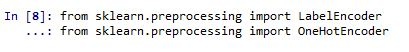
\includegraphics[scale=0.7]{figures/prak5roza.jpg}
\caption{In 5 Roza}
\label{in5roza}
\end{figure}
\par Baris 1: Import labelEncoder dari sklearn.processing digunakan untuk menormalkan label dimana label encoder hanya didefinisikan dengan nilai antara 0 dan n\_classes-1.
\par Baris 2: Memasukkan modul / fungsi OneHotEncoder dari sklearn.processing yang digunakan untuk mendefinisikan fitur input dimana mengambil nilai dalam kisaran [0, maks (nilai)).
\end{itemize}
\par

\item Jelaskan kode program pada blok \# In[6].
\begin{itemize}
\item Kode Program:
\lstinputlisting[firstline=1, lastline=19, caption=Praktek5.py, label={lst:import}]{src/1164085/prak6-roza.py}
\par Hasil \ref{in6roza} :
\begin{figure}[!hbtp]
\centering
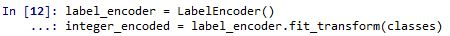
\includegraphics[scale=0.7]{figures/prak6roza.jpg}
\caption{In 6 Roza}
\label{in6roza}
\end{figure}
\par Baris 1: Membuat variabel label\_encoder dengan penerapan modul / fungsi dari LabelEncoder tanpa parameter
\par Baris 2: Membuat variabel integer\_encoded dengan penerapan fungsi label\_encoder.fit\_transform (ekstrasi fitur object ) dari variabel classes dimana akan mengembalikan beberapa data yang diubah kembali dari variabel label\_encoder.
\end{itemize}
\par

\end{enumerate}








\section{Fadila-1164072}
\subsection{Teori}
Penjelasan Tugas Harian 12 ( No 1-11 ).
\begin{enumerate}
\item Mengapa File Teks Harus Dilakukan Tokenizer Besera Ilustrasi Gambar :
\begin{itemize}
\item Tokenizer :
\par Difungsikan untuk membuat vektor dari text. Lebih detailnya, tokenizer merupakan langkah pertama yang diperlukan dalam banyak tugas pemrosesan bahasa alami, seperti penghitungan kata, penguraian, pemeriksaan ejaan, pembuatan corpus, dan analisis statistik teks.
\par
\par
\item Mengapa Text Harus Dilakukan Tokenizer ? :
\par Text harus dilakukan tokenizer agar dapat dirubah menjadi vektor. Dari perubahan ke vektor tersebut maka data/textnya dapat dibaca oleh komputer (terkomputerisasi).
\par
\par
\item Ilustrasi Gambar ( Contoh ): \ref{chapter-7-tokenizer-fadila}
\par
\begin{figure}[!hbtp]
\centering
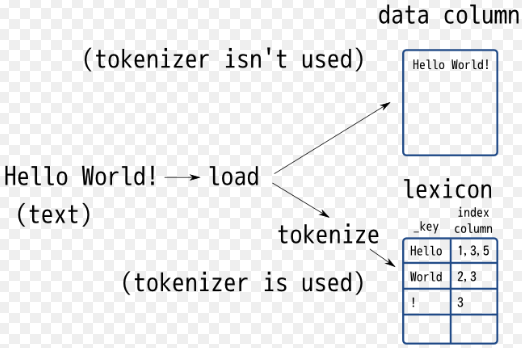
\includegraphics[scale=0.2]{figures/chapter-7-tokenizer-fadila.png}
\caption{Tokenizer - fadila}
\label{chapter-7-tokenizer-fadila}
\end{figure}
\par
\end{itemize}
\par
\par
\item Konsep Dasar K Fold Cross Validation Pada Dataset Komentar Youtube Pada Kode Listing 1 Beserta Dengan Ilustrasi Gambar :
\begin{itemize}
\item Code		:
\lstinputlisting[firstline=8, lastline=20,caption=K Fold Cross Validation,label={lst:7.0}]{src/1164072/teori/chapter-7-2-fadila.py}
\item Penjelasan	: 
\par Untuk kejelasan dari StartifiedKFold yang dicontohkan ialah digunakan dan berisikan presentasi sampel untuk setiap kelas yang ada ( youtube). Pada ilusrasinya sampel dibagi menjadi 5 dalam setiap kelas yang diproses. Kemudian sampelnya sendiri akan dimasukan kedalam class dari dataset youtube yang digunakan.
\par
\item Ilustrasi Gambar ( Contoh ): \ref{chapter-7-starfied-k-fold-cross-fadila}
\par
\par
\begin{figure}[!hbtp]
\centering
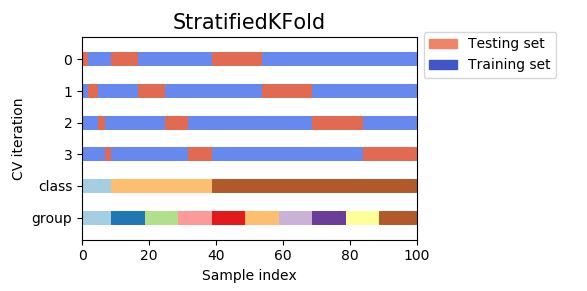
\includegraphics[scale=0.2]{figures/chapter-7-starfied-k-fold-cross-fadila.jpg}
\caption{Startified K-Fold Cross - fadila}
\label{chapter-7-starfied-k-fold-cross-fadila}
\end{figure}
\par
\par
\end{itemize}
\par
\par
\par
\item Jelaskan Apa Maksud Kode Program For Train Dan Test In Splits Dilengkapi Dengan Ilustrasi Gambar :
\begin{itemize}
\item Penjelasan	:
\par Kode Program For Train dan Test In Splits sendiri digunakan ataupun difungsikan untuk pengujian. Pegujiannya yaitu menguji apakah setiap data pada dataset yang dieksekusi sudah di split dan tidak terjadi penumpukan pada data tersebut. Dengan tidak terjadinya penumpukan seperti hal tersebut maka setiap class nya tidak akan memunculkan id yang sama.
\par 
\par
\par
\item Ilustrasi Kalimat ( Contoh ):
\par Dimisalkan dengan contoh dimana terdapat 6 meja dengan model / desain yang berbeda.Langkah selanjutnya dilakukan pendistribusian terhadap meja-meja tersebut kepada 3 investor ( penjual ) maka setiap penjual tersebut tidak akan menjual model meja yang sama dipasaran.
\par
\item Ilustrasi Gambar ( Contoh Lainnya ): \ref{chapter-7-test-in-splits-fadila}
\par
\begin{figure}[!hbtp]
\centering
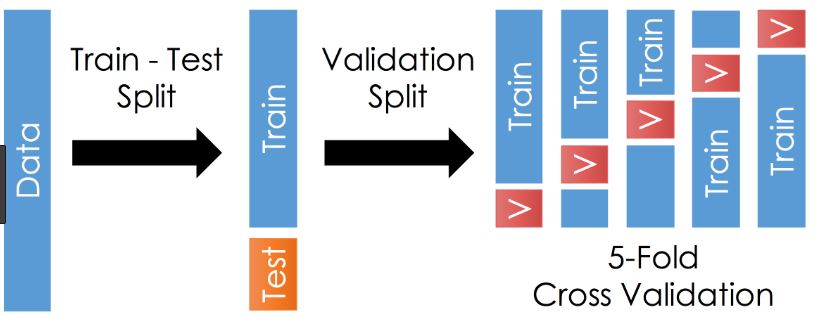
\includegraphics[scale=0.2]{figures/chapter-7-test-in-splits-fadila.jpg}
\caption{chapter-7-test-in-splits-fadila}
\label{chapter-7-test-in-splits-fadila}
\end{figure}
\par
\par
\end{itemize}
\par
\par
\par
\item Apa Maksud Kode Program\emph{train\_content = d['CONTENT'].iloc[train\_idx]} dan \emph{test\_content = d['CONTENT'].iloc[test\_idx]}. Dilengkapi Dengan Ilustrasi Gambar :
\begin{itemize}
\item Penjelasan	:
\par Maksud dari code program tersebut ialah difungsikan dalam pengambilan data pada kolom atau index CONTENT. index Content tersebut merupakan bagian dari train\_idx dan test\_idx. Dengan pendefinisian dan pengaplikasian index Content tersebut pada bagian training data dan test data akan dilakukan pengambilan data yang sesuai dan sama.
\par
\par
\item Ilustrasi Kalimat ( Contoh ):
\par Jika dicontohkan dengan sebuah penjelasan maka bisa dikatakan apabila index CONTENT tersebut direalisasikan maka untuk data yang telah diubah menjadi training data maupun test data bisa dipilih kolom ataupun nilai apa yang akan ditampilkan dan dieksekusi sesuai dengan kebetuhan ataupun keinginan.
\par
\par 
\item Ilustrasi Gambar ( Contoh Lainnya ): \ref{chapter-7-iloc-fadila}
\par Apabila ingin dicontohkan dengan contoh yang lain, dapat dilihat pada gambar berikut dimana contoh ini lebih sederhana hanya menjelaskan tentang penerapan d.iloc yang lebih simple sehingga apabila diterapkan dengan parameter / fungsi lain seperti content dapat lebih dimudah untuk dikerjakan ( berdasarkan basicnya )
\par
\begin{figure}[!hbtp]
\centering
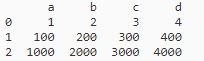
\includegraphics[scale=0.45]{figures/chapter-7-iloc-fadila.jpg}
\caption{Contoh Penerapan .Iloc- fadila}
\label{chapter-7-iloc-fadila}
\end{figure}
\par
\par
\end{itemize}
\par
\par
\par
\item Apa Maksud Dari Fungsi \emph{Tokenizer = Tokenizer(num words=2000) Dan Tokenizer.fit on texts(train content)}, Dilengkapi Dengan Ilustrasi Gambar :
\begin{itemize}
\item Penjelasan	:
\par  Fungsi dari Tokenizer diatas ialah untuk melakukan vektorisasi kata tentunya. Fungsi tokenizer ini mengeksekusi jumlah data yang akan diubah sebesar 2000 kata. 
\par Kemudian untuk  \emph{tokenizer.fit\_on\_texts(train\_content)} digunakan untuk melakukan fit tokenizer. Fungsi tersebut hanya direalisasikan pada data train dan tidak untuk data test kemudian hanya dalam / untuk kolom content seperti yang diperlihatkan pada codingannya.
\item Ilustrasi Kalimat ( Contoh ):
\par Jika dicontohkan dengan sebuah penjelasan maka bisa dikatakan apabila ada kata seperti " My Name Is Far " , " My Name Is ", " Your Name Is ", jika dibuatkan atau dijalankan dengan perintah yang dikatan sama maka akan nampak hasilnya seperti { 'far': 4, 'is' : 1, 'my' : 3, 'name' : 2, 'your':5 } .
\par
\par
\par
\item Ilustrasi Gambar ( Contoh Lainnya ): \ref{chapter-7-tokenizer-sum-words-fadila}
\par
\par
\begin{figure}[!hbtp]
\centering
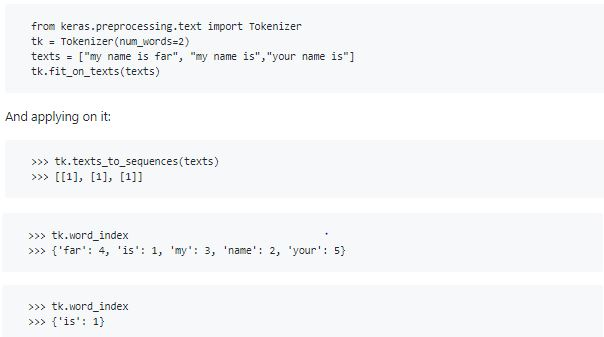
\includegraphics[scale=0.2]{figures/chapter-7-tokenizer-sum-words-fadila.jpg}
\caption{Tokenizer Fit On Text- fadila}
\label{chapter-7-tokenizer-sum-words-fadila}
\end{figure}
\par
\par
\end{itemize}
\par
\par
\par
\item Apa Maksud Dari Fungsi code berikut ( \emph{d\_train\_inputs = tokenizer.texts\_to\_matrix(train\_content, mode='tfidf')} dan \emph{d\_test\_inputs = tokenizer.texts\_to\_matrix(test\_content, mode='tfidf')} ), Dilengkapi Dengan Ilustrasi Kode Dan Atau Gambar :
\begin{itemize}
\item Penjelasan	:
\par Dapat dikatakan bahwa maksud dari codingan diatas ialah untuk variabel d\_train\_inputs dimana akan melakukan tokenizer dari bentuk teks ke / menjadi matrix dari data train\_content menggunakan mode matriks. Mode matriksnya sendiri yaitu tfidf, dan pengaplikasian mode ini juga digunakan untuk dengan variabel d\_test\_inputs untuk data test.
\par
\par
\item Ilustrasi Code Dan Gambar	( Contoh ): \ref{chapter-7-tokenizer-text-matrix-fadila}
\lstinputlisting[firstline=8, lastline=20]{src/1164072/teori/chapter-7-6-fadila.py}
\par
\par
\begin{figure}[!hbtp]
\centering
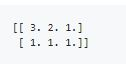
\includegraphics[scale=0.7]{figures/chapter-7-tokenizer-text-matrix-fadila.jpg}
\caption{Tokenizer Text To Matrix- fadila}
\label{chapter-7-tokenizer-text-matrix-fadila}
\end{figure}
\par
\par
\end{itemize}
\par
\par
\par
\item Jelaskan Apa Maksud Dari Fungsi Berikut ( \emph{d\_train\_inputs = d\_train\_inputs/np.amax(np.absolute(d\_train\_inputs))} dan \emph{d\_test\_inputs = d\_test\_inputs/np.amax(np.absolute(d\_test\_inputs))} ) Kemudian Dilengkapi Dengan Ilustrasi Gambar :
\begin{itemize}
\item Penjelasan : 
\par Berdasarkan code diatas, menjelaskan bahwa fungsi tersebut akan membagi matrix tfidf yang sudah dieksekusi sebelumnya dengan amax. Amaxnya sendiri berfungsi dalam pengembalian maksimum array atau maksimum sepanjang sumbu. Untuk hasilnya akan dimasukan kedalam variabel d\_train\_inputs untuk data train dan d\_test\_inputs untuk data test berupa nilai absolute atautanpa ada bilangan negatif.
\par
\par
\item Ilustrasi Code Dan Gambar	( Contoh ): \ref{chapter-7-np-amax-fadila} dan \ref{chapter-7-np-absolute-fadila}
\begin{itemize}
\item Contoh 1 :
\lstinputlisting[firstline=8, lastline=20]{src/1164072/teori/chapter-7-7-amax-fadila.py}
\par
\par
\par
\begin{figure}[!hbtp]
\centering
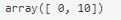
\includegraphics[scale=0.7]{figures/chapter-7-np-amax-fadila.jpg}
\caption{Contoh Penerapan Np Amax- fadila}
\label{chapter-7-np-amax-fadila}
\end{figure}
\par
\item Contoh 2 :
\lstinputlisting[firstline=8, lastline=20]{src/1164072/teori/chapter-7-7-absolute-fadila.py}
\par
\par
\begin{figure}[!hbtp]
\centering
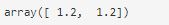
\includegraphics[scale=0.7]{figures/chapter-7-np-absolute-fadila.jpg}
\caption{Contoh Penerapan Np Absolute- fadila}
\label{chapter-7-np-absolute-fadila}
\end{figure}
\par
\end{itemize}
\end{itemize}
\par
\par
\item Jelaskan Apa Maksud Dari \emph{d\_train\_outputs = np.utils.to\_categorical(d['CLASS'].iloc[train]} Dan \emph{d\_test\_outputs = np\_utils.to\_categorical(d['CLASS'].iloc[test\_idx]} Dalam Kode Program Dilengkapi Dengan Ilustrasi Gambar :
\begin{itemize}
\item Penjelasan : 
\par Yang dimaksudkan dari kode program tersebut dapat dijelaskan bahwa fungsnya ditujukan untuk melakukan one-hot encoding. One-hot encoding itu direalisasikan supaya bisa masuk dan digunakan pada neural network. 
\par One-hot encoding diambil dari 'CLASS' yang berarti hanya terdapat 2 neuron, yaitu dengan nilai satu nol(1,0) atau nol satu(0,1). Mengapa demikian? dikarenakan pilihannya hanya ada dua yaitu spam atau bukan spam.
\par
\par
\item Ilustrasi Code Dan Gambar	( Contoh ): \ref{chapter-7-np-utils-to-categorical-fadila}
\lstinputlisting[firstline=8, lastline=20]{src/1164072/teori/chapter-7-8-fadila.py}
\par
\begin{figure}[!hbtp]
\centering
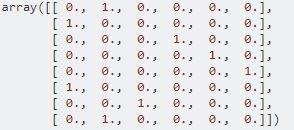
\includegraphics[scale=0.6]{figures/chapter-7-np-utils-to-categorical-fadila.jpg}
\caption{Contoh Penerapan Np.utils.to categorical - fadila}
\label{chapter-7-np-utils-to-categorical-fadila}
\end{figure}
\par
\par
\end{itemize}
\par
\par
\par
\item Jelaskan Maksud Dari Fungsi Di Listing 7.2. Gambarkan Ilustrasi Neural Networknya Dari Model Kode Tersebut.
\begin{itemize}
\item Code :
\lstinputlisting[firstline=8, lastline=20]{src/1164072/teori/chapter-7-9-fadila.py}
\item Penjelasan : 
\par Berdasarkan code tersebut, dimaksudkan atau ditujukan untuk melakukan pemodelan dengan sequential. Sequential tersebut untuk membandingkan setiap satu larik elemen dengan cara satu persatu secara beruntun. Terdapat 512 neuron inputan dengan input shape 2000 vektor yang sudah dinormalisasi. 
\par Selanjutnya model dilakukan aktivasi dengan fungsi 'relu', yang setelahnya terjadi pemotongan bobot  sebesar 50 persen dari neuron inputan 512 ( agar tidak overfitting ). Pada layer output terdapat 2 neuron outputan yaitu nol(1,0) atau nol satu(0,1). Setelah semua ketentuan tersebut, dimunculkan outputan yang diaktivasi menggunakan fungsi softmax.
\par
\par
\end{itemize}
\par
\par
\par
\par
\item Jelaskan Maksud Dari Fungsi Di Listing 7.3. Dengan Parameter Berikut :
\begin{itemize}
\item Code :
\lstinputlisting[firstline=8, lastline=20]{src/1164072/teori/chapter-7-10-fadila.py}
\item Penjelasan : 
\par Berdasarkan code tersebut , dimaksudkan bahwa model yang telah dibuat akan dicompile dengan menggunakan algoritma optimisasi (adamax), fungsi loss(categorical\_crossentropy), dan fungsi metrik untuk perhitungan akurasinya.
\par
\par
\end{itemize}
\par
\par
\par
\item Apa itu Deep Learning :
\begin{itemize}
\item Penjelasan :
\par Deep learning merupakan sub bidang pembelajaran mesin yang berkaitan dengan algoritma yang terinspirasi oleh struktur dan fungsi otak yang disebut jaringan saraf tiruan.
\par
\par
\par
\end{itemize}
\item Apa itu Deep Neural Network Dan Apa Bedanya Dengan Deep Learning :
\begin{itemize}
\item Penjelasan Deep Neural Network : 
\par Deep neural network adalah jaringan syaraf dengan tingkat kompleksitas tertentu, jaringan syaraf dengan lebih dari dua lapisan. Deep neural netwok menggunakan pemodelan matematika yang canggih untuk memproses data dengan cara yang kompleks.
\par
\item Perbedaan Deep Neural Network Dan Deep Learning :
\par Perbedaan antara deep neural network dan deep learning terletak pada kedalaman model. deep learning adalah frasa yang digunakan untuk jaringan saraf yang kompleks. Kompleksitas ini disebabkan oleh pola yang rumit tentang bagaimana informasi dapat mengalir di seluruh model. Arsitekturnya menjadi lebih kompleks tetapi konsep deep learning masih sama. Meskipun sekarang ada peningkatan jumlah layer dan node tersembunyi yang terintegrasi untuk memperkirakan output.
\par Untuk pemahaman yang lebih baik, diberikan sebuah contoh terkait dengan penjelasan perbedaan antara deep neural network dan deep learning.
\par
\par
\item Ilustrasi Gambar ( Contoh ): \ref{chapter-7-beda-deep-neu-dan-deep-learn-fadila}
\par
\par
\begin{figure}[!hbtp]
\centering
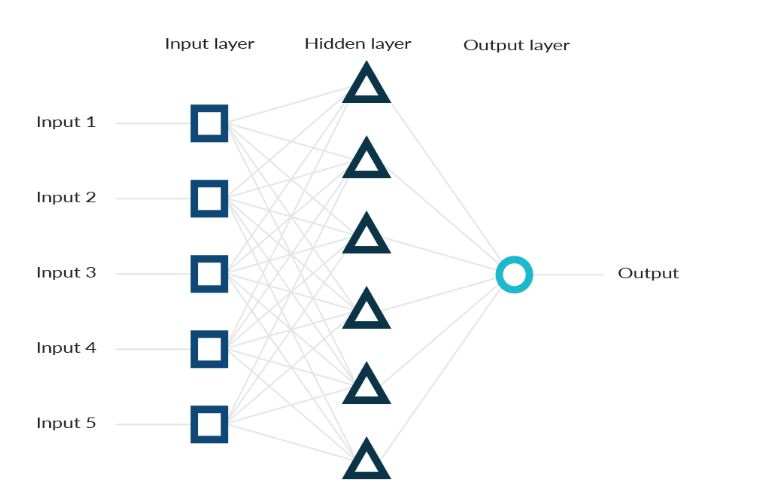
\includegraphics[scale=0.2]{figures/chapter-7-beda-deep-neu-dan-deep-learn-fadila.jpg}
\caption{Perbedaan Deep NW Dan Deep Learn- fadila}
\label{chapter-7-beda-deep-neu-dan-deep-learn-fadila}
\end{figure}
\par
\par
\end{itemize}
\par
\par
\item Bagaimana Perhitungan Algoritma Dengan Ukuran Stride (NPM mod3+1)x(NPM mod3+1) Yang  Terdapat Pada Max Pooling :
\begin{itemize}
\item Penjelasan :
\par Konvolusi pada sebuah gambar dilakukan dalam image processing untuk menerapkan operator yang mempunyai nilai output dari piksel gambar yang berasal dari kombinasi linear nilai input piksel tertentu pada gambar.
\par
\item Langkah-langkah Algoritma Konvulasi Sesuai NPM : \ref{chapter-7-algoritma-konvolusi-fadila}
\par
\par
\begin{figure}[!hbtp]
\centering
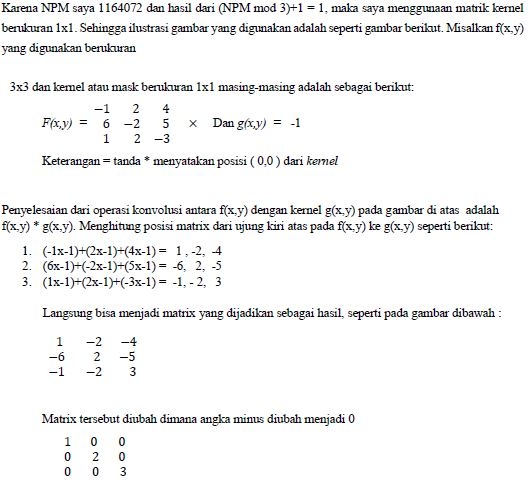
\includegraphics[scale=0.52]{figures/chapter-7-algoritma-konvolusi-fadila.jpg}
\caption{Langkah Algoritma Konvolusi Berdasarkan NPM- fadila}
\label{chapter-7-algoritma-konvolusi-fadila}
\end{figure}
\par
\par
\end{itemize}
\end{enumerate}

\begin{itemize}
\item  Plagiarisme Fadila: \ref{chapter-7-plagiarisme-fadila}
\par
\begin{figure}[!hbtp]
\centering
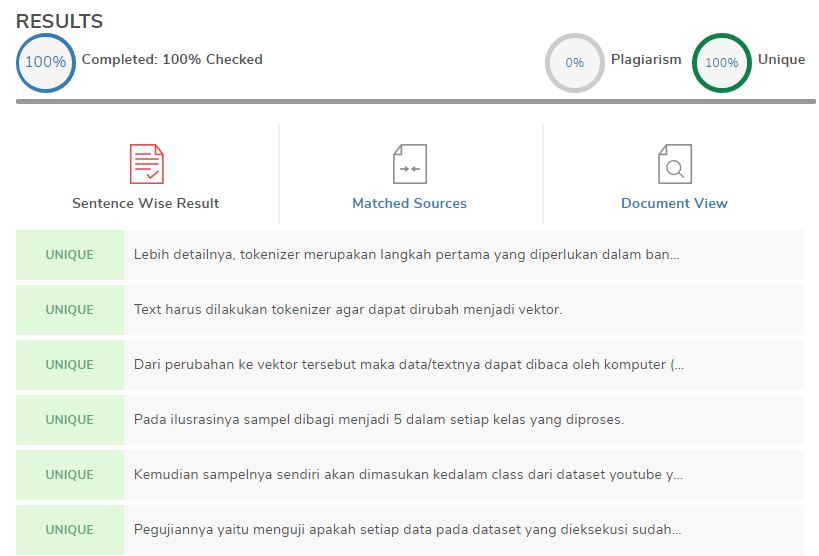
\includegraphics[scale=0.3]{figures/chapter-7-plagiarisme-fadila.jpg}
\caption{Plagiarisme- fadila}
\label{chapter-7-plagiarisme-fadila}
\end{figure}
\par
\par
\end{itemize}


\par
\par
\par
\par
\subsection{Praktek}
Penjelasan Tugas Harian 12 ( No 1-20 ).
\begin{enumerate}
\item Jelaskan Kode Program Pada Blok \# In[1]. Jelaskan Arti Dari Setiap Baris Kode Yang Dibuat Dan Hasil Keluarannya Dari Komputer Sendiri.
\begin{itemize}
\item Code Yang Digunakan : \ref{lst:chapter-7-1-fadila}.
\lstinputlisting[firstline=1, lastline=19,caption=File chapter-7-1-fadila.py, label={lst:chapter-7-1-fadila}]{src/1164072/praktek/chapter-7-1-fadila.py}
\par
\par
\item Penjelasan Code Perbaris	: 
\begin{enumerate}
\item Baris Code 1	: Memasukkan / Mengimport file csv
\item Baris Code 2	: Memasukkan module image sebagai pil\_image dari library PIL dimana PIL dapat mendukung pembukaan, pemanipulasian, dan menyimpan banyak format file gambar yang berbeda
\item Baris Code 3	: Memasukkan / mengimport fungsi keras.processing.image 
\end{enumerate}
\par
\item Hasil : \ref{chapter-7-in-1-fadila}
\par
\par
\begin{figure}[!hbtp]
\centering
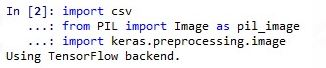
\includegraphics[scale=0.4]{figures/chapter-7-in-1-fadila.jpg}
\caption{Code Program Pada In [1] - fadila}
\label{chapter-7-in-1-fadila}
\end{figure}
\par
\par
\end{itemize}
\par
\par
\par
\item Jelaskan Kode Program Pada Blok \# In[2]. Jelaskan Arti Dari Setiap Baris Kode Yang Dibuat Dan Hasil Keluarannya Dari Komputer Sendiri.
\begin{itemize}
\item Code Yang Digunakan : \ref{lst:chapter-7-2-fadila}.
\lstinputlisting[firstline=1, lastline=19,caption=File chapter-7-2-fadila.py, label={lst:chapter-7-2-fadila}]{src/1164072/praktek/chapter-7-2-fadila.py}
\par
\par
\item Penjelasan Code Perbaris	: 
\begin{enumerate}
\item Baris Code 1	: Membuat variabel imgs tanpa parameter
\item Baris Code 2	: Membuat variabel classes tanpa parameter
\item Baris Code 3	: Membuka file HASYv2/hasy-data-labels.csv sebagai csvfile
\item Baris Code 4	: Membuat variabel csvreader yang memfungsikan pembacaan dari file csv yang dimasukkan
\item Baris Code 5	: Membuat variabel i dengan parameter 0
\item Baris Code 6	: Mengeksekusi baris dari pembacaan csv 
\item Baris Code 7	: Mengaplikasikan perintah "if" dengan ketentuan variabel i lebih besar dari angka 0, maka akan dilanjutkan ke perintah berikutnya
\item Baris Code 8	: Membuat variabel img yang mengubah image menjadi bentuk array (bilangan) dari file HASYv2 yang dibuka dengan row berparameter 0.
\item Baris Code 9	: Membuat variabel img tidak sama dengan nilai 255.0
\item Baris Code 10	: Mendefinisikan fungsi imgs.append dimana merupakan proses melampirkan atau menggabungkan data dengan file lain atau set data yang ditentukan dengan 3 parameter yaitu row[0], row[2] dan variabel img.
\item Baris Code 11	: Mendefinisikan fungsi append kembali dari variabel classes dengan parameternya row[2].
\item Baris Code 12	: Mendefinisikan fungsi dimana i variabel i akan ditambah nilainya sehingga akan bernilai 1 ( 0 dengan penambahan maka akan jadi 1 )
\end{enumerate}
\par
\item Hasil : \ref{chapter-7-in-2-fadila}
\par
\par
\begin{figure}[!hbtp]
\centering
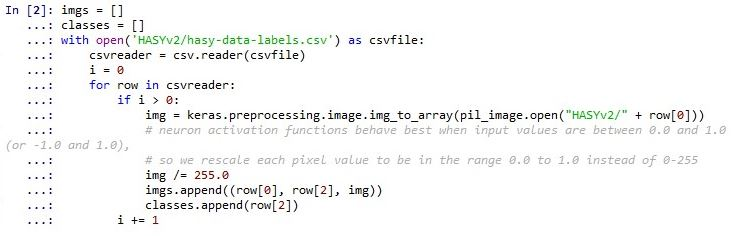
\includegraphics[scale=0.4]{figures/chapter-7-in-2-fadila.jpg}
\caption{Code Program Pada In [2] - fadila}
\label{chapter-7-in-2-fadila}
\end{figure}
\par
\par
\end{itemize}
\par
\par
\par
\item Jelaskan Kode Program Pada Blok \# In[3]. Jelaskan Arti Dari Setiap Baris Kode Yang Dibuat Dan Hasil Keluarannya Dari Komputer Sendiri.
\begin{itemize}
\item Code Yang Digunakan : \ref{lst:chapter-7-3-fadila}.
\lstinputlisting[firstline=1, lastline=19,caption=File chapter-7-3-fadila.py, label={lst:chapter-7-3-fadila}]{src/1164072/praktek/chapter-7-3-fadila.py}
\par
\par
\item Penjelasan Code Perbaris	: 
\begin{enumerate}
\item Baris Code 1	: Memasukkan dan memfungsikan module random
\item Baris Code 2	: Melakukan pengocokan pada module random dengan parameter variabelnya imgs
\item Baris Code 3	: Membagi dan memecah index dalam bentuk integer dengan mengkalikannilai 0,8 dan fungsi len yang akan mengembalikan jumlah item dalam datanya dari variabel imgs
\item Baris Code 4	: Membuat variabel train yang mengeksekusi imgs dengan pemecahan index awal pada data
\item Baris Code 5	: Membuat variabel test yang mengeksekusi imgs dengan pemecahan index akhir pada data
\end{enumerate}
\par
\item Hasil : \ref{chapter-7-in-3-fadila}
\par
\par
\begin{figure}[!hbtp]
\centering
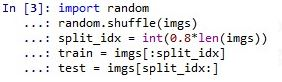
\includegraphics[scale=0.4]{figures/chapter-7-in-3-fadila.jpg}
\caption{Code Program Pada In [3] - fadila}
\label{chapter-7-in-3-fadila}
\end{figure}
\par
\par
\end{itemize}
\par
\par
\par
\item Jelaskan Kode Program Pada Blok \# In[4]. Jelaskan Arti Dari Setiap Baris Kode Yang Dibuat Dan Hasil Keluarannya Dari Komputer Sendiri.
\begin{itemize}
\item Code Yang Digunakan : \ref{lst:chapter-7-4-fadila}.
\lstinputlisting[firstline=1, lastline=19,caption=File chapter-7-4-fadila.py, label={lst:chapter-7-4-fadila}]{src/1164072/praktek/chapter-7-4-fadila.py}
\par
\par
\item Penjelasan Code Perbaris	: 
\begin{enumerate}
\item Baris Code 1	: Memasukkan / Mengimport library numpy sebagai np
\item Baris Code 2	: Membuat variabel train\_input dimana mengubah input menjadi sebuah array dari np dengan menggunakan fungsi list untuk mengkoleksikan data yang dipilih dan dapat diubah. Didalamnya diterapkan fungsi map untuk mengembalikan iterator dari datanya dengan memfungsikan lamda pada row dengan parameter [2] untuk membuat objek fungsi menjadi lebih kecil dan mudah dieksekusi dari variabel train.
\item Baris Code 3	: Membuat variabel test\_input dengan fungsi yang sama seperti train\_input yang membedakan hanya datanya / inputan yang diproses berasal dari variabel test
\item Baris Code 4	: Membuat variabel train\_output dimana mengubah keluaran menjadi sebuah array dari np dengan menggunakan fungsi list untuk mengkoleksikan data yang dipilih dan dapat diubah. Didalamnya diterapkan fungsi map untuk mengembalikan iterator dari datanya dengan memfungsikan lamda pada row dengan parameter[1] untuk membuat objek fungsi menjadi lebih kecil dan mudah dieksekusi dari variabel train.
\item Baris Code 5	: Membuat variabel test\_output dengan fungsi yang sama seperti train\_output yang membedakan hanya datanya / inputan yang diproses berasal dari variabel test
\end{enumerate}
\par
\item Hasil : \ref{chapter-7-in-4-fadila}
\par
\par
\begin{figure}[!hbtp]
\centering
\includegraphics[scale=0.4]{figures/chapter-7-in-4-fadila.jpg}
\caption{Code Program Pada In [4] - fadila}
\label{chapter-7-in-4-fadila}
\end{figure}
\par
\par
\end{itemize}
\par
\par
\par
\item Jelaskan Kode Program Pada Blok \# In[5]. Jelaskan Arti Dari Setiap Baris Kode Yang Dibuat Dan Hasil Keluarannya Dari Komputer Sendiri.
\begin{itemize}
\item Code Yang Digunakan : \ref{lst:chapter-7-5-fadila}.
\lstinputlisting[firstline=1, lastline=19,caption=File chapter-7-5-fadila.py, label={lst:chapter-7-5-fadila}]{src/1164072/praktek/chapter-7-5-fadila.py}
\par
\par
\item Penjelasan Code Perbaris	: 
\begin{enumerate}
\item Baris Code 1	: Memasukkan modul / fungsi LabelEncoder dari sklearn.processing yang digunakan untuk dapat  menormalkan label dimana label encoder hanya didefinisikan dengan nilai antara 0 dan -1.
\item Baris Code 2	: Memasukkan modul / fungsi OneHotEncoder dari sklearn.processing yang digunakan untuk mendefinisikan fitur input dimana mengambil nilai dalam kisaran [0, maks (nilai)).
\end{enumerate}
\par
\item Hasil : \ref{chapter-7-in-5-fadila}
\par
\par
\begin{figure}[!hbtp]
\centering
\includegraphics[scale=0.4]{figures/chapter-7-in-5-fadila.jpg}
\caption{Code Program Pada In [5] - fadila}
\label{chapter-7-in-5-fadila}
\end{figure}
\par
\par
\end{itemize}
\par
\par
\par
\item Jelaskan Kode Program Pada Blok \# In[6]. Jelaskan Arti Dari Setiap Baris Kode Yang Dibuat Dan Hasil Keluarannya Dari Komputer Sendiri.
\begin{itemize}
\item Code Yang Digunakan : \ref{lst:chapter-7-6-fadila}.
\lstinputlisting[firstline=1, lastline=19,caption=File chapter-7-6-fadila.py, label={lst:chapter-7-6-fadila}]{src/1164072/praktek/chapter-7-6-fadila.py}
\par
\par
\item Penjelasan Code Perbaris	: 
\begin{enumerate}
\item Baris Code 1	: Membuat variabel label\_encoder dengan penerapan modul / fungsi dari LabelEncoder tanpa parameter
\item Baris Code 2	: Membuat variabel integer\_encoded dengan penerapan fungsi label\_encoder.fit\_transform (ekstrasi fitur object ) dari variabel classes yang akan mengembalikan beberapa data yang diubah kembali.
\end{enumerate}
\par
\item Hasil : \ref{chapter-7-in-6-fadila}
\par
\par
\begin{figure}[!hbtp]
\centering
\includegraphics[scale=0.4]{figures/chapter-7-in-6-fadila.jpg}
\caption{Code Program Pada In [6] - fadila}
\label{chapter-7-in-6-fadila}
\end{figure}
\par
\par
\end{itemize}
\par
\par
\par
\item Jelaskan Kode Program Pada Blok \# In[7]. Jelaskan Arti Dari Setiap Baris Kode Yang Dibuat Dan Hasil Keluarannya Dari Komputer Sendiri.
\begin{itemize}
\item Code Yang Digunakan : \ref{lst:chapter-7-7-fadila}.
\lstinputlisting[firstline=1, lastline=19,caption=File chapter-7-7-fadila.py, label={lst:chapter-7-7-fadila}]{src/1164072/praktek/chapter-7-7-fadila.py}
\par
\par
\item Penjelasan Code Perbaris	: 
\begin{enumerate}
\item Baris Code 1	:
\item Baris Code 2	:
\item Baris Code 3	:
\item Baris Code 4	:
\item Baris Code 5	:
\item Baris Code 6	:
\item Baris Code 7	:
\end{enumerate}
\end{itemize}
\par
\par
\par
\item Jelaskan Kode Program Pada Blok \# In[8]. Jelaskan Arti Dari Setiap Baris Kode Yang Dibuat Dan Hasil Keluarannya Dari Komputer Sendiri.
\begin{itemize}
\item Code Yang Digunakan : \ref{lst:chapter-7-8-fadila}.
\lstinputlisting[firstline=1, lastline=19,caption=File chapter-7-8-fadila.py, label={lst:chapter-7-8-fadila}]{src/1164072/praktek/chapter-7-8-fadila.py}
\par
\par
\item Penjelasan Code Perbaris	: 
\begin{enumerate}
\item Baris Code 1	:
\item Baris Code 2	:
\item Baris Code 3	:
\item Baris Code 4	:
\item Baris Code 5	:
\item Baris Code 6	:
\item Baris Code 7	:
\end{enumerate}
\end{itemize}
\par
\par
\par
\item Jelaskan Kode Program Pada Blok \# In[9]. Jelaskan Arti Dari Setiap Baris Kode Yang Dibuat Dan Hasil Keluarannya Dari Komputer Sendiri.
\begin{itemize}
\item Code Yang Digunakan : \ref{lst:chapter-7-9-fadila}.
\lstinputlisting[firstline=1, lastline=19,caption=File chapter-7-9-fadila.py, label={lst:chapter-7-9-fadila}]{src/1164072/praktek/chapter-7-9-fadila.py}
\par
\par
\item Penjelasan Code Perbaris	: 
\begin{enumerate}
\item Baris Code 1	:
\item Baris Code 2	:
\item Baris Code 3	:
\item Baris Code 4	:
\item Baris Code 5	:
\item Baris Code 6	:
\item Baris Code 7	:
\end{enumerate}
\par
\end{itemize}
\par
\par
\par
\item Jelaskan Kode Program Pada Blok \# In[10]. Jelaskan Arti Dari Setiap Baris Kode Yang Dibuat Dan Hasil Keluarannya Dari Komputer Sendiri.
\begin{itemize}
\item Code Yang Digunakan : \ref{lst:chapter-7-10-fadila}.
\lstinputlisting[firstline=1, lastline=19,caption=File chapter-7-10-fadila.py, label={lst:chapter-7-10-fadila}]{src/1164072/praktek/chapter-7-10-fadila.py}
\par
\par
\item Penjelasan Code Perbaris	: 
\begin{enumerate}
\item Baris Code 1	:
\item Baris Code 2	:
\item Baris Code 3	:
\item Baris Code 4	:
\item Baris Code 5	:
\item Baris Code 6	:
\item Baris Code 7	:
\end{enumerate}
\par
\end{itemize}
\par
\par
\par
\item Jelaskan Kode Program Pada Blok \# In[11]. Jelaskan Arti Dari Setiap Baris Kode Yang Dibuat Dan Hasil Keluarannya Dari Komputer Sendiri.
\begin{itemize}
\item Code Yang Digunakan : \ref{lst:chapter-7-11-fadila}.
\lstinputlisting[firstline=1, lastline=19,caption=File chapter-7-11-fadila.py, label={lst:chapter-7-11-fadila}]{src/1164072/praktek/chapter-7-11-fadila.py}
\par
\par
\item Penjelasan Code Perbaris	: 
\begin{enumerate}
\item Baris Code 1	:
\item Baris Code 2	:
\item Baris Code 3	:
\item Baris Code 4	:
\item Baris Code 5	:
\item Baris Code 6	:
\item Baris Code 7	:
\end{enumerate}
\par
\end{itemize}
\par
\par
\par
\item Jelaskan Kode Program Pada Blok \# In[12]. Jelaskan Arti Dari Setiap Baris Kode Yang Dibuat Dan Hasil Keluarannya Dari Komputer Sendiri.
\begin{itemize}
\item Code Yang Digunakan : \ref{lst:chapter-7-12-fadila}.
\lstinputlisting[firstline=1, lastline=19,caption=File chapter-7-12-fadila.py, label={lst:chapter-7-12-fadila}]{src/1164072/praktek/chapter-7-12-fadila.py}
\par
\par
\item Penjelasan Code Perbaris	: 
\begin{enumerate}
\item Baris Code 1	:
\item Baris Code 2	:
\item Baris Code 3	:
\item Baris Code 4	:
\item Baris Code 5	:
\item Baris Code 6	:
\item Baris Code 7	:
\end{enumerate}
\par
\end{itemize}
\par
\par
\par
\item Jelaskan Kode Program Pada Blok \# In[13]. Jelaskan Arti Dari Setiap Baris Kode Yang Dibuat Dan Hasil Keluarannya Dari Komputer Sendiri.
\begin{itemize}
\item Code Yang Digunakan : \ref{lst:chapter-7-13-fadila}.
\lstinputlisting[firstline=1, lastline=19,caption=File chapter-7-13-fadila.py, label={lst:chapter-7-13-fadila}]{src/1164072/praktek/chapter-7-13-fadila.py}
\par
\par
\item Penjelasan Code Perbaris	: 
\begin{enumerate}
\item Baris Code 1	:
\item Baris Code 2	:
\item Baris Code 3	:
\item Baris Code 4	:
\item Baris Code 5	:
\item Baris Code 6	:
\item Baris Code 7	:
\end{enumerate}
\par
\end{itemize}
\par
\par
\par
\item Jelaskan Kode Program Pada Blok \# In[14]. Jelaskan Arti Dari Setiap Baris Kode Yang Dibuat Dan Hasil Keluarannya Dari Komputer Sendiri.
\begin{itemize}
\item Code Yang Digunakan : \ref{lst:chapter-7-14-fadila}.
\lstinputlisting[firstline=1, lastline=19,caption=File chapter-7-14-fadila.py, label={lst:chapter-7-14-fadila}]{src/1164072/praktek/chapter-7-14-fadila.py}
\par
\par
\item Penjelasan Code Perbaris	: 
\begin{enumerate}
\item Baris Code 1	:
\item Baris Code 2	:
\item Baris Code 3	:
\item Baris Code 4	:
\item Baris Code 5	:
\item Baris Code 6	:
\item Baris Code 7	:
\end{enumerate}
\par
\par
\end{itemize}
\par
\par
\par
\item Jelaskan Kode Program Pada Blok \# In[15]. Jelaskan Arti Dari Setiap Baris Kode Yang Dibuat Dan Hasil Keluarannya Dari Komputer Sendiri.
\begin{itemize}
\item Code Yang Digunakan : \ref{lst:chapter-7-15-fadila}.
\lstinputlisting[firstline=1, lastline=19,caption=File chapter-7-15-fadila.py, label={lst:chapter-7-15-fadila}]{src/1164072/praktek/chapter-7-15-fadila.py}
\par
\par
\item Penjelasan Code Perbaris	: 
\begin{enumerate}
\item Baris Code 1	:
\item Baris Code 2	:
\item Baris Code 3	:
\item Baris Code 4	:
\item Baris Code 5	:
\item Baris Code 6	:
\item Baris Code 7	:
\end{enumerate}
\par
\end{itemize}
\par
\par
\par
\item Jelaskan Kode Program Pada Blok \# In[16]. Jelaskan Arti Dari Setiap Baris Kode Yang Dibuat Dan Hasil Keluarannya Dari Komputer Sendiri.
\begin{itemize}
\item Code Yang Digunakan : \ref{lst:chapter-7-16-fadila}.
\lstinputlisting[firstline=1, lastline=19,caption=File chapter-7-16-fadila.py, label={lst:chapter-7-16-fadila}]{src/1164072/praktek/chapter-7-16-fadila.py}
\par
\par
\item Penjelasan Code Perbaris	: 
\begin{enumerate}
\item Baris Code 1	:
\item Baris Code 2	:
\item Baris Code 3	:
\item Baris Code 4	:
\item Baris Code 5	:
\item Baris Code 6	:
\item Baris Code 7	:
\end{enumerate}
\par
\end{itemize}
\par
\par
\par
\item Jelaskan Kode Program Pada Blok \# In[17]. Jelaskan Arti Dari Setiap Baris Kode Yang Dibuat Dan Hasil Keluarannya Dari Komputer Sendiri.
\begin{itemize}
\item Code Yang Digunakan : \ref{lst:chapter-7-17-fadila}.
\lstinputlisting[firstline=1, lastline=19,caption=File chapter-7-17-fadila.py, label={lst:chapter-7-17-fadila}]{src/1164072/praktek/chapter-7-17-fadila.py}
\par
\par
\item Penjelasan Code Perbaris	: 
\begin{enumerate}
\item Baris Code 1	:
\item Baris Code 2	:
\item Baris Code 3	:
\item Baris Code 4	:
\item Baris Code 5	:
\item Baris Code 6	:
\item Baris Code 7	:
\end{enumerate}
\par
\par
\end{itemize}
\par
\par
\par
\item Jelaskan Kode Program Pada Blok \# In[18]. Jelaskan Arti Dari Setiap Baris Kode Yang Dibuat Dan Hasil Keluarannya Dari Komputer Sendiri.
\begin{itemize}
\item Code Yang Digunakan : \ref{lst:chapter-7-18-fadila}.
\lstinputlisting[firstline=1, lastline=19,caption=File chapter-7-18-fadila.py, label={lst:chapter-7-18-fadila}]{src/1164072/praktek/chapter-7-18-fadila.py}
\par
\par
\item Penjelasan Code Perbaris	: 
\begin{enumerate}
\item Baris Code 1	:
\item Baris Code 2	:
\item Baris Code 3	:
\item Baris Code 4	:
\item Baris Code 5	:
\item Baris Code 6	:
\item Baris Code 7	:
\end{enumerate}
\par
\par
\end{itemize}
\par
\par
\par
\item Jelaskan Kode Program Pada Blok \# In[19]. Jelaskan Arti Dari Setiap Baris Kode Yang Dibuat Dan Hasil Keluarannya Dari Komputer Sendiri.
\begin{itemize}
\item Code Yang Digunakan : \ref{lst:chapter-7-19-fadila}.
\lstinputlisting[firstline=1, lastline=19,caption=File chapter-7-19-fadila.py, label={lst:chapter-7-19-fadila}]{src/1164072/praktek/chapter-7-19-fadila.py}
\par
\par
\item Penjelasan Code Perbaris	: 
\begin{enumerate}
\item Baris Code 1	:
\item Baris Code 2	:
\item Baris Code 3	:
\item Baris Code 4	:
\item Baris Code 5	:
\item Baris Code 6	:
\item Baris Code 7	:
\end{enumerate}
\par
\par
\end{itemize}
\par
\par
\par
\item Jelaskan Kode Program Pada Blok \# In[20]. Jelaskan Arti Dari Setiap Baris Kode Yang Dibuat Dan Hasil Keluarannya Dari Komputer Sendiri.
\begin{itemize}
\item Code Yang Digunakan : \ref{lst:chapter-7-20-fadila}.
\lstinputlisting[firstline=1, lastline=19,caption=File chapter-7-20-fadila.py, label={lst:chapter-7-20-fadila}]{src/1164072/praktek/chapter-7-20-fadila.py}
\par
\par
\item Penjelasan Code Perbaris	: 
\begin{enumerate}
\item Baris Code 1	:
\item Baris Code 2	:
\item Baris Code 3	:
\item Baris Code 4	:
\item Baris Code 5	:
\item Baris Code 6	:
\item Baris Code 7	:
\end{enumerate}
\par
\end{itemize}
\par
\par
\par
\end{enumerate}


\subsection{Penanganan Error}
Penjelasan Tugas Harian 12 ( No 1-20 ).
\begin{enumerate}
\item Error 1	:
\begin{itemize}
\item Screenshoot Error 	: \ref{chapter-7-error-1-fadila}
\par
\par
\begin{figure}[!hbtp]
\centering
\includegraphics[scale=0.2]{figures/chapter-7-error-1-fadila.jpg}
\caption{Error 1 - fadila}
\label{chapter-7-error-1-fadila}
\end{figure}
\par
\item Code Error		:
\begin{lstlisting}
ModuleNotFoundError: No module named 'tensorflow'
\end{lstlisting}
\item Penanganan Error	:
\begin{enumerate}
\item Pertama-tama pastikan salahnya seperti apa ( model dan jenis errornya )
\item Kemudian, silahkan proses error tersebut dengan cara yang sesuai
\item Berdasarkan error maka penyelesaiannya ialah melakukan instalasi terhadap module 'tensorflow' sehingga code dapat dijalankan
\item Buka Anaconda Prompt kemudian lakukan perintah seperti pada gambar berikut ( conda install -c conda-forge tensorflow ) : \ref{chapter-7-penanganan-error-1-fadila}
\par
\begin{figure}[!hbtp]
\centering
\includegraphics[scale=0.2]{figures/chapter-7-penanganan-error-1-fadila.jpg}
\caption{Penanganan Error 1 - fadila}
\label{chapter-7-penanganan-error-1-fadila}
\end{figure}
\par
\item Setelah melakukan perintah berikut maka silahkan jalankan kembali code maka tidak akan terjadi lagi error tersebut.
\end{enumerate}
\end{itemize}
\par
\par
\item Error 2 :
\begin{itemize}
\item Screenshoot Error 	: \ref{chapter-7-error-2-fadila}
\par
\par
\begin{figure}[!hbtp]
\centering
\includegraphics[scale=0.2]{figures/chapter-7-error-2-fadila.jpg}
\caption{Error 2 - fadila}
\label{chapter-7-error-2-fadila}
\end{figure}
\par
\item Code Error		:
\begin{lstlisting}
NameError: name 'model' is not defined
\end{lstlisting}
\item Penanganan Error	:
\begin{enumerate}
\item Pertama-tama pastikan salahnya seperti apa ( model dan jenis errornya )
\item Kemudian, silahkan proses error tersebut dengan cara yang sesuai
\item Berdasarkan error maka penyelesaiannya ialah melakukan pendefinisian variabel model sehingga code dapat dijalankan
\par
\begin{figure}[!hbtp]
\centering
\includegraphics[scale=0.2]{figures/chapter-7-penanganan-error-2-fadila.jpg}
\caption{Penanganan Error 2 - fadila}
\label{chapter-7-penanganan-error-2-fadila}
\end{figure}
\par
\item Setelah melakukan pendefinisian variabel tersebut maka silahkan jalankan kembali code maka tidak akan terjadi lagi error tersebut.
\end{enumerate}
\end{itemize}
\end{enumerate}